% !TEX root = ../CA_book.tex

\chapter{복소미분}

이 장에서는 다음 3가지 주제를 중점적으로 다룬다.

\begin{itemize}
\item[(1)] 복소미분의 정의:
즉, $\mathbb C$의 열린 부분집합 $U$에 정의된 함수 $f:U\to\mathbb C$와
$z_0\in U$가 주어졌을 때, ``$f$가 $z_0$에서 복소미분가능하고 복소미분값은 $f'(z_0)$이다''
라는 의미에 대하여 학습한다.
\item[(2)] 코시-리만 방정식: 
$\dfrac{\partial u}{\partial x} = \dfrac{\partial v}{\partial y}$와
$\dfrac{\partial u}{\partial y} = - \dfrac{\partial v}{\partial x}$.

이 방정식은 
복소미분가능함수 $f:U\to\mathbb C$의 실수부와 허수부 $u$, $v$가
만족하는 편미분방정식이다.

\begin{figure}[!h]
\begin{center}
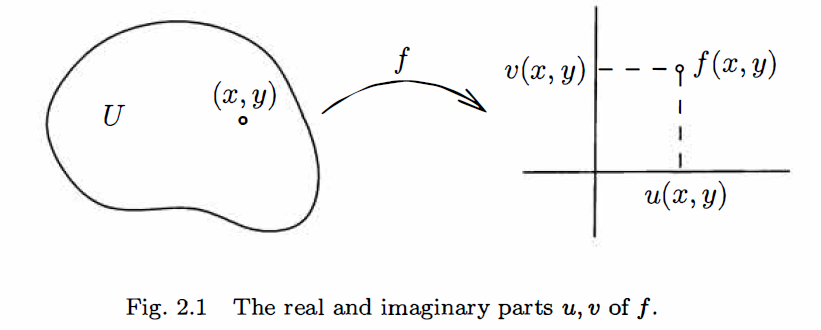
\includegraphics[width=0.6\textwidth]{./SaltChapter/fig-2-1}
\end{center}
\caption{$f$의 실수부와 허수부 $u$, $v$}
\label{fig-2-1}
\end{figure}

역으로, 어떤 열린집합 $U$의 모든 점에서 $C^1$-함수 $u, v$가 
코시-리만 방정식을 만족한다면 $f=u+iv$는 $U$에서 복소미분가능하다.

\item[(3)] 복소미분 $f'(z_0)$의 기하학적 의미:
국소적으로 보면, 함수 $f$는 $|f'(z_0)|$만큼 확대하면서
반시계방향으로 $\Arg(f'(z_0))$만큼 회전시키는 변환이다.
\end{itemize}

이 장에서는
열린집합에 정의된 복소미분가능함수가 
코시-리만 방정식을 만족할 필요충분조건(다소 덜 엄밀한 방식으로)에 대하여
중점적으로 다룬다.

\section{복소 미분가능성}

\begin{saltdefinition} {}{}\label{def-2-1}

\begin{itemize}
\item[(1)] $U$가 $\mathbb C$의 열린 부분집합, $f: U\to \mathbb C$, $z_0\in U$라 하자.
다음 식을 만족하는 복소수 $L$이 존재하면, $f$가 $z_0$에서 {\bf 복소미분가능}이라 한다.
\[
\lim_{z\to z_0} \dfrac{f(z) - f(z_0)}{z - z_0} = L.
\]
즉, 임의의 $\epsilon>0$에 대하여 $\delta>0$가 존재하여,
$z\in U$, $0<|z-z_0|<\delta$이면 
\[
\left| \dfrac{f(z) - f(z_0)}{z - z_0} - L\right| < \epsilon
\]
을 만족한다.

극한값  $L$은 유일하게 결정되며 다음과 같이 나타낸다.
\[
f'(z_0) \quad\text{또는}\quad \dfrac{df}{dz}(z_0).
\]

\item[(2)] 열린집합 $U$에 정의된 함수 $f:U\to\mathbb C$가 $U$의 모든 점에서
복소미분가능하면 복소해석적(holomorphic\footnote{
``holomorphic''이라는 용어는 전체(entire)를 뜻하는 그리스어 ``holo''와
``모양(form)'' 또는 ``형세(apprearance)''을 나타내는 ``morphe''에서 파생되었다.
})이라 부른다.
\item[(3)] 복소수 $\mathbb C$ 전체에서 복소해석적이면 
전해석(entire) 함수라 부른다. 즉, $f$의 정의역이 복소수 $\mathbb C$ 전체이고
$\mathbb C$에서 복소해석적임을 의미한다.
\end{itemize}
\end{saltdefinition}

전해석 함수의 간단한 예를 살펴보자.

\begin{saltexample}[label=example-2-1]{}{example-2-1} 
함수 $f:\mathbb C \to \mathbb C$를 $f(z) = z^2$ ($z\in\mathbb C$)라 정의하자.
그러면 $f$가 전해석 함수임을 보일 수 있다.
$z$가 $z_0$의 근방에 있을 때,
\[
\dfrac{f(z) - f(z_0)}{z - z_0} = \dfrac{z^2 - z_0^2}{z-z_0} = z + z_0 
\approx 2z_0
\]
이므로, $f'(z_0) = 2z_0$라고 추측할 수 있다.
이를 증명해 보자.
$z\ne z_0$에 대하여
\[
\left| \dfrac{f(z) - f(z_0)}{z - z_0} - 2z_0 \right|
= \left| \dfrac{z^2 - z_0^2}{z-z_0} - 2z_0 \right| 
= |z+z_0-2z_0| = |z-z_0|.
\]
따라서 $z$가 $z_0$에 충분히 가까우면
좌변을 원하는 만큼 작은 값으로 만들 수 있다.
$\epsilon>0$이라 하자.
$\delta:=\epsilon>0$으로 잡으면,
$z\in\mathbb C$가 $0<|z-z_0| <\delta$를 만족할 때마다
\[
\left| \dfrac{f(z) - f(z_0)}{z - z_0} - 2z_0 \right|
= |z-z_0| <\delta = \epsilon.
\]
결론적으로 $f'(z_0) = 2z_0$가 성립한다.
$z_0\in\mathbb C$를 임의로 선택할 수 있으므로,
$f$는 $\mathbb C$ 전체에서 복소해석적이고,
전해석 함수가 된다. 이상에서 다음 결론을 얻는다.
\[
\dfrac{d}{dz} z^2 = 2z, \quad z\in \mathbb C.
\]
\end{saltexample}

다른 방향으로, 이제 복소미분가능하지 않은 함수의 예를 보자.

\begin{saltexample}[label=example-2-2]{}{}
함수 $g:\mathbb C \to \mathbb C$를 $g(z) = \bar z$ ($z\in\mathbb C$)라 정의하자.
그러면 $g$는 어떤 점에서도 복소미분이 불가능함을 보일 수 있다.
$g$가 $z_0\in\mathbb C$에서 복소미분가능하다고 하자.
$\epsilon:=\frac12 >0$라 하면, $\delta>0$이 존재하여
$z$가 $0<|z-z_0|<\delta$를 만족할 때마다 
\[
\left| \dfrac{g(z)-g(z_0)}{z-z_0} - g'(z_0) \right| 
= \left| \dfrac{\bar z - \overline{z_0}}{z-z_0} - g'(z_0) \right| 
<\epsilon
\]
이 성립한다.

그림 \ref{fig-2-2}의 왼쪽을 보자.
위의 식에 따르면,
중심이 $z_0$이고 반지름이 $\delta$인 뚫린 원판(punctured disk)에 $z$가 속할 때마다
부등식이 성립함을 보장한다.
이제 그림의 뚫린 원판 내부에 $z_0$의 위쪽과 오른쪽에 한점씩을 선택하자.
이 점들을 부등식에 넣어보면, $g'(z_0)$는 각각 $-1$과 $1$을 중심으로 하고 반지름 $1/2$인
원판 내부에 속해야 한다.
그림 \ref{fig-2-2}의 오른쪽을 참고하면, 두 원판은 겹치치 않으므로 모순이 되어 증명이 끝난다.
아래에서 좀 더 자세히 살펴보자.

%\begin{figure}[!h]
\begin{center}
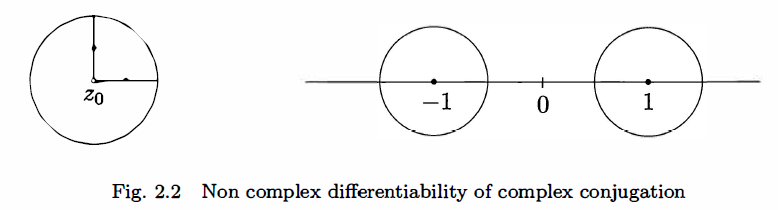
\includegraphics[width=0.8\textwidth]{./SaltChapter/fig-2-2}
\end{center}
\captionof{figure}{켤레복소수 함수의 미분 불가능성}
\label{fig-2-2}
%\end{figure}

$z=z_0+ \dfrac\delta2$로 잡으면, $0<|z-z_0|<\delta$이므로
\begin{equation} \label{eq-2-1}
\left| \dfrac{\bar z - \overline{z_0}}{z-z_0} - g'(z_0) \right| 
= \left| \dfrac{\delta/2}{\delta/2} - g'(z_0) \right| 
= | 1 - g'(z_0)| < \epsilon.
\end{equation}
한편, $z=z_0+ i\dfrac\delta2$로 잡으면, $0<|z-z_0|<\delta$이므로
\begin{equation} \label{eq-2-2}
\left| \dfrac{\bar z - \overline{z_0}}{z-z_0} - g'(z_0) \right| 
= \left| \dfrac{-\delta/2}{\delta/2} - g'(z_0) \right| 
= | 1 + g'(z_0)| < \epsilon.
\end{equation}
식 \eqref{eq-2-1}과 \eqref{eq-2-2}로부터
\[
2 = | 1- g'(z_0) + 1+ g'(z_0)|
\le |1-g'(z_0)| + |1+g'(z_0)| < \epsilon + \epsilon 
= 2\epsilon = 2\cdot\dfrac12 = 1
\]
이 되어 모순이다.
따라서 $g$는 $z_0$에서 복소미분가능하지 않다.
\end{saltexample}

\begin{salt_exercise} \label{ex-2-1}
모든 $z\in\mathbb C$에 대하여 $f(z) = |z|^2$로 정의된
함수 $f:\mathbb C \to \mathbb C$는 $0$에서 복소미분가능하며
$f'(0)=0$임을 보여라.
나중에 (연습문제 \ref{ex-2-9}에서) $f$는 $0$이 아닌 모든 점에서 복소미분 불가능함을 보일 것이다.
\end{salt_exercise}

\begin{salt_exercise} \label{ex-2-2}
영역 $D$에 정의된 함수 $f:D\to \mathbb C$가 복소해석적이라 하자.
$D^* := \{ z\in \mathbb C \,:\, \bar z \in D\}$에 
함수 $f^*:D^* \to \mathbb C$를 $f^*(z) = \overline{f(\bar  z)}$ ($z\in D^*$)로
정의하면 $f^*$가  $D^*$에서 복소해석적임을 증명하라.
\end{salt_exercise}

복소미분 가능성에 대한 다음 변형은 복소미분에 대한 기본 공식을 증명하는 데 유용하게 사용된다.
대략적으로 말하면, 복소미분가능함수 $f$가 $z_0$에서 미분값 $L$을 갖는다면
$f(z)-f(z_0) - L\cdot (z-z_0)$가 $z-z_0$보다 $0$으로 빠르게 수렴함을 뜻한다.

\begin{salt_lemma} \label{lemma-2-1}
$U$가 $\mathbb C$의 열린 집합이고, $z_0\in U$, $f:U\to\mathbb C$라 하면,
다음은 동치이다.
\begin{itemize}
\item[(1)] $f$가 $z_0$에서 복소미분가능하며, $f'(z_0)=L$이다.
\item[(2)] 양수 $r>0$과  $D(z_0,r):=\{z\in\mathbb C\,:\, |z-z_0|<r\}$에 정의된
함수  $h:D(z_0,r)\to \mathbb C$가 존재하여 다음을 만족한다.
\begin{itemize}
\item[(a)] $|z-z_0|<r$에 대하여 $f(z)=f(z_0) + (L+h(z))(z-z_0)$이고,
\item[(b)] $\lim\limits_{z\to z_0} h(z)=0$.
\end{itemize}
\end{itemize}
\end{salt_lemma}

{\bf 증명}

(2)$\Rightarrow$(1):
$z\in D(z_0,r)\setminus \{z_0\}$에 대하여 (a)의 식을 재정리하면,
\[
\dfrac{f(z) - f(z_0)}{z - z_0} - L = h(z) \stackrel{z\to z_0}{\longrightarrow} 0
\]
이므로 $f$는 $z_0$에서 복소미분가능하며 $f'(z_0)=L$이다.

(1)$\Rightarrow$(2):
이제 $f$가 $z_0$에서 복소미분가능하다고 가정하자. 
그러면 $\delta_1>0$이 존재하여 \\
$0<|z-z_0|<\delta_1$, $z\in U$이면 
\[
\left|  \dfrac{f(z) - f(z_0)}{z - z_0}  - f'(z_0) \right| < 1
\]
이다.
$r:=\delta_1$으로 설정하고 함수 $h:D(z_0,r) \to \mathbb C$를 
\[
h(z) = \begin{cases}
\dfrac{f(z) - f(z_0)}{z - z_0} - f'(z_0), & z\ne z_0, \\
0, & z= z_0
\end{cases}
\]
로 정의하자.
그러면 $|z-z_0|<r$일 때
$f(z) = f(z_0) + \left( f'(z_0) + h(z)\right) (z - z_0)$가 성립한다.
이제 (b)를 보이기 위해 $\epsilon>0$이 주어졌다고 하자.
$0<|z-z_0|<\delta$이면
\[
\left|  \dfrac{f(z) - f(z_0)}{z - z_0}  - f'(z_0) \right| \ \left( = |h(z) - 0| \right) < \epsilon
\]
이 되는 $\delta>0$를 잡을 수 있다 ($r$보다 작다는 조건도 만족하도록).
이로써 (a), (b)를 모두 성립함을 알 수 있다. \hfill $\square$

\begin{salt_exercise} \label{ex-2-3}
영역 $D\subset \mathbb C$에 정의된 함수 $f:D\to \mathbb C$가 
$z_0\in D$에서 복소미분가능하다면 $f$는 $z_0$에서 연속임을 보여라.
나중에 우리는 $f$가 $D$에서 복소해석적이면, 
실제로 $D$의 모든 점에서 무한번 미분가능함을 보일 것이다.
\end{salt_exercise}

보조정리 \ref{lemma-2-1}을 이용하여 다음을 쉽게 얻을 수 있다.

\begin{saltprop}{}{} \label{prop-2-1}
$U$가 $\mathbb C$의 열린 부분집합이고,
$f,g: U\to \mathbb C$가 $z_0\in U$에서 복소미분가능함수이면
다음이 성립한다.
\begin{itemize}
\item[(1)] $f+g$는 $z_0$에서 복소미분가능하고
$(f+g)'(z_0) = f'(z_0) = g'(z_0)$이다. \\
(함수 $f+g:U\to\mathbb C$는 $z\in U$에 대하여 $(f+g)(z) = f(z)+g(z)$로 정의한다)
\item[(2)] $\alpha\in\mathbb C$에 대하여 $\alpha\cdot f$는 $z_0$에서 복소미분가능하고
$(\alpha\cdot f)'(z_0) = \alpha f'(z_0)$이다. \\
(함수 $\alpha \cdot f:U\to\mathbb C$는 $z\in U$에 대하여 
$(\alpha \cdot f)(z) = \alpha f(z)$로 정의한다)
\item[(3)] $fg$는 $z_0$에서 복소미분가능하고
$(fg)'(z_0) = f'(z_0)g(z_0) + f(z_0)g'(z_0)$이다.\\
(함수 $fg:U\to\mathbb C$는 $z\in U$에 대하여 
$(fg)(z)= f(z)g(z)$로 정의한다)
\end{itemize}
\end{saltprop}

\begin{salt_remark}\label{remark-2-1}
$U$가 $\mathbb C$의 열린 부분집합이고,
$\Hol(U)$가 $U$에 정의된 복소해석 함수의 집합이라고 하자.
그러면 위 명제로부터 $\Hol(U)$가 점별 연산에 대하여 복소 벡터공간을 이룸을 알 수 있다.
한편 위 명제의 세번째 내용은 두 복소해석 함수의 점별 곱셈은 다시 복소해석적임을 뜻한다.
따라서 $\Hol(U)$는 점별 덧셈과 곱셈에 대하여
환(ring) 구조를 갖는다.
\end{salt_remark}

\begin{saltexample}[label=example-2-3]{}{}
$f(z):=z$ ($z\in \mathbb C$)에 대하여 $f'(z)=1$임을 쉽게 보일 수 있다.
두 복소해석함수의 점별 곱셈에 대한 복소미분 규칙을 이용하면,
수학적 귀납법으로 모든 $n\in \mathbb N$에 $z\mapsto z^n$이 전해석함수이고
\[
\dfrac{d}{dz} z^n = nz^{n-1}
\]
임을 알 수 있다.
특히, 모든 다항식은 전해석함수이다.
\end{saltexample}

\begin{salt_exercise} \label{ex-2-4}
명제 \ref{prop-2-1}\을 증명하라.
\end{salt_exercise}


\begin{salt_exercise} \label{ex-2-5}
$\mathbb D = \{ z\in\mathbb C \,:\, |z|<1 \}$이고
$\Hol(\mathbb D)$가 $\mathbb D$에 정의된 복소해석함수의 점별 연산으로 이루어진
복소 벡터공간이라 하자.  $\Hol(\mathbb D)$는 유한차원인가?
\end{salt_exercise}


\begin{salt_exercise} \label{ex-2-6}
$U$가 $\mathbb C$의 열린 부분집합이고,
$U$에 정의된 복소해석함수 $f:U\to \mathbb C$가 
$z\in U$에 대하여 $f(z)\ne 0$라고 하자.
\[
\dfrac 1f : U \to \mathbb C \text{ 를 }
\left( \dfrac 1f \right) (z) = \dfrac 1{f(z)} \text{ 로 정의할 때 }
\]
복소해석함수가 되며 복소미분이 다음과 같음을 보여라.
\[
\left( \dfrac 1f \right)' (z) = - \dfrac{f'(z)}{(f(z))^2} \quad (z\in U).
\]
\end{salt_exercise}

\begin{salt_exercise} \label{ex-2-7}
$\mathbb C\setminus \{0\}$에서 정수 $m\in\mathbb Z$에 대하여
$\dfrac d{dz} z^m = mz^{m-1}$임을 증명하라.
\end{salt_exercise}

실수에서 정의된 합성함수의 미분에 대한 연쇄법식과 같이
복소해석함수의 합성에 대해서도 유사한 연쇄법식이 존재한다.

\begin{saltprop}[연쇄법칙]{}{} \label{prop-2-2} 
\begin{itemize}
\item[(1)] $D_f$, $D_g$가 복소평면 위의 영역이고,
\item[(2)] $f:D_f \to \mathbb C$가 $D_f$에서 복소해석적이고,
\item[(3)] $g:D_g \to \mathbb C$가 $D_g$에서 복소해석적이고,
\item[(4)] $f(D_f) \subset D_g$일 때,
\end{itemize}
$z\in D_f$에 대하여 $(g\circ f)(z) = g(f(z))$로 정의된
합성함수 $g\circ f : D_f \to \mathbb C$는 $D_f$에서
복소해석함수이고, 
모든 $z\in D_f$에 대하여 $(g\circ f)'(z) = g'(f(z))f'(z)$이다.
\end{saltprop}

\begin{figure}[!h]
\begin{center}
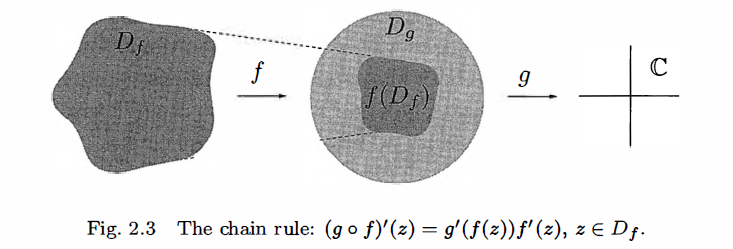
\includegraphics[width=0.7\textwidth]{./SaltChapter/fig-2-3}
\end{center}
\caption{연쇄법칙: $z\in D_f$에 대하여 $(g\circ f)'(z) = g'(f(z))f'(z)$}
\label{fig-2-3}
\end{figure}

{\bf 증명}

$z_0\in D_f$라 하자. 그러면 $f(z_0)\in D_g$이다.
$f$가 $z_0$의 근방에서 복소미분가능하고
$g$가 $f(z_0)$의 근방에서 복소미분가능하므로,
원판 $D(z_0, r_f)\subset D_f$와 $D(f(z_0), r_g) \subset D_g$에 각각 정의된
함수 $h_f$와 $h_g$가 존재하여 다음을 만족한다.
\begin{gather*}
f(z) - f(z_0) = (f'(z_0)+h_f(z))(z-z_0), \\
g(w) - g(f(z_0)) = (g'(f(z_0)) + h_g(w))(w-f(z_0)),
\end{gather*}
또한
\[
\lim_{z\to z_0} h_f(z)=0, \quad
\lim_{w\to f(z_0)} h_g(w)=0.
\]
$f$가 $z_0$에서 연속이므로
$z$가 $z_0$에 가까워질 때 $w:=f(z)$도 $f(z_0)$에 가까워지므로
$z\ne z_0$이고 $z_0$에 가까워지면, 다음 식을 얻는다.
\[
\dfrac{(g\circ f)(z) - (g\circ f)(z_0)}{z-z_0} 
= (g'(f(z_0)) + h_g(f(z)))(f'(z_0) + h_f(z)).
\]
이로써 증명이 끝난다. \hfill $\square$

\begin{saltexample}[label=example-2-4]{}{}
연습문제 \ref{ex-2-7}로부터
\[
\dfrac d{dz} \left(\dfrac 1z \right) = - \dfrac 1{z^2}, \quad
z\in \mathbb C \setminus \{0\}
\]
임을 알지만, 복소미분 정의로부터도의 쉽게 유도할 수 있다. 왜냐 하면,
$z_0\in \mathbb C \setminus \{0\}$에 대하여 다음 식이 성립하기 때문이다.
\[
\dfrac{\dfrac 1z - \dfrac1{z_0}}{z-z_0} = \dfrac{z_0 - z}{zz_0(z-z_0)}
= \dfrac{-1}{zz_0} \stackrel{z\to z_0}{\longrightarrow} - \dfrac 1{z_0^2}.
\] 
%\begin{figure}[!h]
\begin{center}
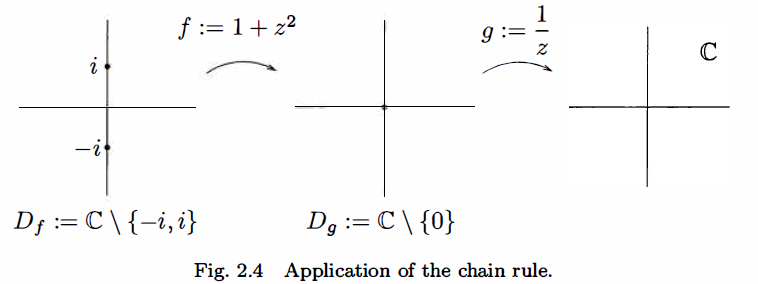
\includegraphics[width=0.7\textwidth]{./SaltChapter/fig-2-4}
\end{center}
\captionof{figure}{연쇄법칙의 응용}
\label{fig-2-4}
%\end{figure}
이제 $D_f:=\mathbb C \setminus \{-i,i\}$에 정의된 함수 $f:= 1+z^2$와
$D_g:=\mathbb C \setminus \{0\}$에 정의된 함수 $g:=1/z$를 생각하자.
$f(D_f) \subset D_g$이 성립함이 명확하므로 연쇄법식에 의해
$\mathbb C \setminus \{-i, i\}$에서
\[
\dfrac d{dz} \left( \dfrac 1{1+z^2} \right) = - \dfrac 1{(1+z^2)^2}\cdot 2z
= - \dfrac{2z}{(1+z^2)^2}.
\]
\end{saltexample}

\begin{salt_exercise} \label{ex-2-8}
$\exp z$가 전해석함수이고 $\exp' z = \exp z$라 가정하고(나중에 증명할 예정이다),
\[
z \mapsto \exp \left( - \dfrac{1+z}{1-z} \right)
\]
가 단위 원판 $\mathbb D := \{ z \in \mathbb C \,:\, |z|<1 \}$에서
복소미분가능함수임을 보이고, 미분을 구하라.
\end{salt_exercise}

\section{코시-리만 방정식}

이제 이 장에서 가장 중요한 결과를 증명해보자.
간략히 말하면, 함수  $f=u+iv$가 복소미분가능하다는 것은
실수부 $u$와 허수부 $v$ ($\mathbb R^2$의 열린 부분집합에 정의된 실함수로 볼 수 있는)가
코시-리만(Cauchy-Riemann) 방정식이라 불리는 편미분 방정식을 만족함과 동치이다. 

\begin{figure*}[!h]
\begin{center}
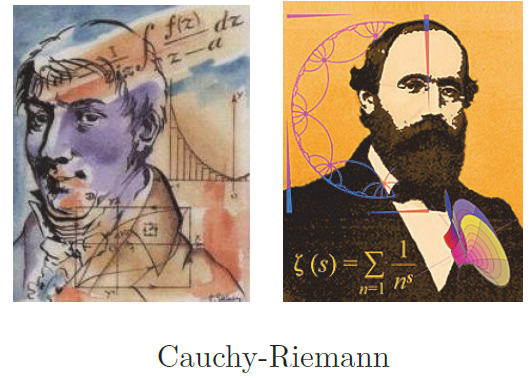
\includegraphics[width=0.4\textwidth]{./SaltChapter/fig-2-0-1} \\
{코시-리만(Cauchy-Riemann)}
\end{center}
%== [salt]?? 캡션을 넣으면 번호가 자동부여?
%\caption{코시-리만(Cauchy-Riemann)}
\end{figure*}


$\mathbb C$의 열린 부분집합 $U$에 정의된
함수 $f:U\to \mathbb C$를 생각하자.
그러면 임의의 점 $(x,y)\in U$에 대하여 $f(x+iy)\in\mathbb C$이고,
$f(x+iy)$의 실수부 $u(x,y)$와 허수부 $v(x,y)$를 그림 \ref{fig-2-5}와 같이 볼 수 있다.

\begin{figure}[!h]
\begin{center}
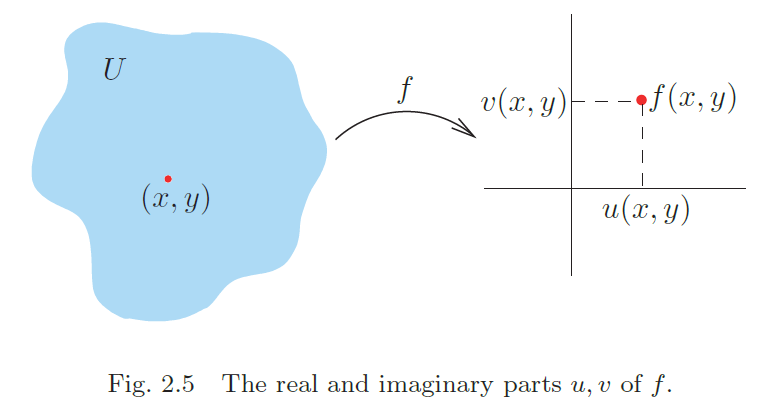
\includegraphics[width=0.6\textwidth]{./SaltChapter/fig-2-5}
\end{center}
\caption{$f$의 실수부 $u$와 허수부 $v$}
\label{fig-2-5}
\end{figure}

점 $(x,y)$가 변하면 $f(x+iy)$도 변하며, $u(x,y)$와 $v(x,y)$도 마찬가지다.
이런 방법으로, $f$와 연관된 실함수를 얻는다.
\begin{align*}
u:U\to \mathbb R, & U \ni (x,y) \mapsto \Re(f(x+iy)) =: u(x,y), \\
v:U\to \mathbb R, & U \ni (x,y) \mapsto \Im(f(x+iy)) =: v(x,y). \\
\end{align*}

이 장의 첫번째 결과는 코시-리만 방정식이 복소미분가능성에 대한 필요조건이라는 것이며
이는 정리 \ref{thm-2-1}에서 증명할 것이다. 
즉, $f$가 $(x_0, y_0) \in U$에서 복소미분가능하다면,

\begin{center}
$(x_0, y_0)$에서
\fbox{
$\dfrac{\partial u}{\partial x} =  \dfrac{\partial v}{\partial y}$ 이고
$\dfrac{\partial u}{\partial y} = - \dfrac{\partial v}{\partial x}$.
}
\end{center}

이를 이 방정식을 코시-리만 방정식이라 부른다.
따라서 복소미분가능함수는 이 방정식을 만족한다.
다시 말하면, 복소함수의 실수부와 허수부가 어떤 점에서 이 방정식을 만족하지 않는다면,
그 점에서 복소미분가능하지 않음을 알 수 있다.
여기서 예제 하나를 보자. 앞에서 우리는 $\epsilon-\delta$를 이용한 복소미분의 정의로부터
직접 계산하여 $z\mapsto \bar z$가 복소평면위의 어느 점에서도 미분가능하지 않음을 보였다.
예제 \ref{example-2-2}를 다시 살펴보자.

\begin{saltexample}[label=example-2-5]{}{}
$g(z) = \bar z$ ($z\in \mathbb C$)로 정의된 함수 $g:\mathbb C \to \mathbb C$에 대하여
\begin{align*}
u(x,y) &=\Re(g(x+iy)) = \Re(x-iy) = x, \\
v(x,y) &= \Im(g(x+iy)) = \Im(x-iy) = -y
\end{align*}
이므로
\[
\dfrac{\partial u}{\partial x} = 1 \ne -1 = \dfrac{\partial v}{\partial y}.
\]
이 결과는 코시-리만 방정식이 어떤 점에서도 성립하지 않음을 의미한다.
따라서 $g$가 어떤 점에서도 복소미분가능하지 않다는 이전 결과를 쉽게 얻을 수 있다.
\end{saltexample}


코시-리만 방정식이 복소미분가능성에 대한 필요조건이라는 것을 증명하기에 앞서
이 절에서 증명할 두번째로 중요한 결과로
열린집합에서 복소해석적일 충분조건으로서
코시-리만 방정식에 대하여 언급하고자 한다.
좀 더 정확히 말하면, 
열린집합 $U$에 정의된 함수 $u,v: U\to \mathbb R$가 
$U$에서 연속미분가능하고 (이변수 실함수로서),
$U$의 모든 점에서 코시-리만 방정식을 만족하면,
$u$, $v$로부터 $f(x+iy):=u(x,y) + iv(x,y)$ $(x,y)\in U$로 정의하여 만든
($u$, $v$가 $f$의 실수부와 허수부가 되도록)
새로운 복소함수 $f:U\to\mathbb C$는 복소해석적이다.
이 중요한 결과로부터 우리는
$\epsilon-\delta$ 정의를 이용하는 매우 긴 증명을 통하지 않고
주요 함수의 복소미분가능성을 확인할 수 있다.
예제를 살펴보자.

\begin{saltexample}[label=example-2-6]{}{}
뚫린 평면 $\mathbb R^2 \setminus \{(0,0)\}$에서 
\[
u(x,y) := \dfrac{x}{x^2+y^2}, \quad
v(x,y) := \dfrac{-y}{x^2+y^2}, \quad (x,y)\ne(0,0)
\]
로 정의된 함수 
$u$, $v$를 생각하자.
그러면 다음 편미분을 얻는다.
\begin{align*}
\dfrac{\partial u}{\partial x} &= \dfrac{1\cdot(x^2+y^2)-x\cdot 2x}{(x^2+y^2)^2}
= \dfrac{y^2-x^2}{(x^2+y^2)^2}, \\
\dfrac{\partial u}{\partial y} &= \dfrac{-x\cdot 2y}{(x^2+y^2)^2}
= \dfrac{-2xy}{(x^2+y^2)^2}, \\
\dfrac{\partial v}{\partial x} &= \dfrac{2xy}{(x^2+y^2)^2}, \quad
\dfrac{\partial v}{\partial y} = \dfrac{y^2-x^2}{(x^2+y^2)^2}.
\end{align*}
당연히 $\mathbb R^2$에서 $(x,y) \mapsto (x^2+y^2)^2, y^2-x^2, \pm 2xy$는 
연속함수이고, $(x^2+y^2)^2$은 $\mathbb R^2 \setminus \{(0,0)\}$에서 
$0$이 아니다.
따라서 $u$, $v$는 $\mathbb R^2 \setminus \{(0,0)\}$에서 
연속미분가능하다.
또한 코시-리만 방정식이 성립한다. 
결론적으로 $f:=u+iv$는 $\mathbb C\setminus\{0\}$에서 
복소해석적이다.
실제로 위에서 정의한 $f$는 다름 아닌 분수함수 $z\mapsto 1/z$이다.
\[
f=u+iv= \dfrac x{x^2+y^2}+i\left(\dfrac{-y}{x^2+y^2}\right)
= \dfrac{x-iy}{x^2+y^2} = \dfrac{\bar z}{|z|^2} = \dfrac{\bar z}{z \bar z}
= \dfrac  1z, \quad z\ne 0.
\]
\end{saltexample}

%\newpage %[salt] 빼면 페이지가 이상함

\begin{salttheorem}{}{} \label{thm-2-1}
$U$가 $\mathbb C$의 열린 부분집합이고
$f:U\to \mathbb C$가 $z_0=x_0+iy_0\in U$에서 복소미분가능하다고 하자.
그러면 함수
\begin{align*}
(x,y) \mapsto u(x,y) & := \Re(f(x+iy)): U\to \mathbb R, \\
(x,y) \mapsto v(x,y) & := \Im(f(x+iy)): U\to \mathbb R
\end{align*}
는 $(x_0, y_0)$에서 미분가능하고 다음을 만족한다.
\begin{equation} \label{eq-2-3}
\dfrac{\partial u}{\partial x}(x_0,y_0) = \dfrac{\partial v}{\partial y}(x_0,y_0),
\quad
\dfrac{\partial u}{\partial y}(x_0,y_0) = - \dfrac{\partial u}{\partial x}(x_0,y_0),.
\end{equation}
\end{salttheorem}

{\bf 증명}
(증명의 아이디어는 쉽다. 단지 $(x,y)$를 $(x_0, y_0)$에 가까이 보낼 때
첫번째로 $y$를 $y_0$로 고정하는 방법으로 하고 그 다음에 
$x$를 $x_0$로 고정하는 방법을 사용한 후 각 결과를 살펴본다.
그림 \ref{fig-2-6}을 참고하라.)

\begin{figure}[!h]
\begin{center}
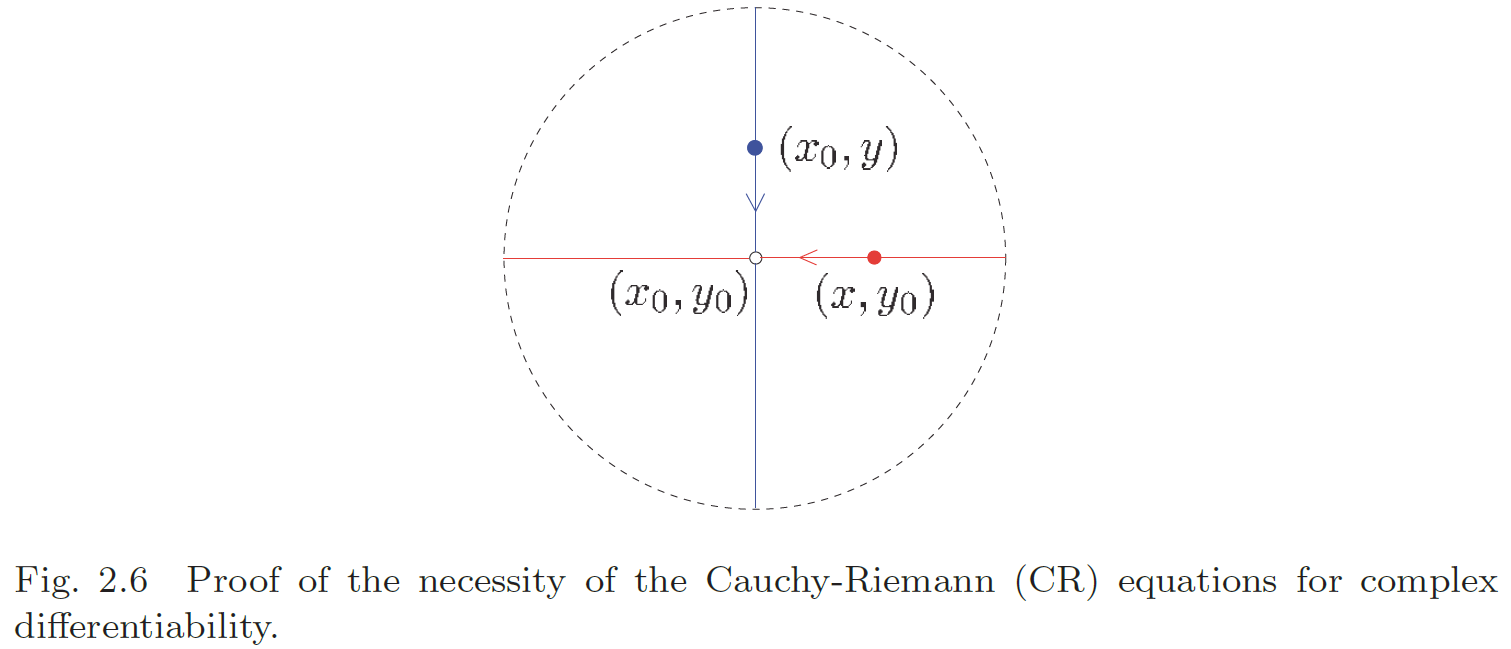
\includegraphics[width=0.9\textwidth]{./SaltChapter/fig-2-6}
\end{center}
\caption{복소미분가능성에 대하여 코시-리만(CR) 방정식이 필요조건임을 증명}
\label{fig-2-6}
\end{figure}

$z_0 = (x_0, y_0)\in U$라 하자.
$\epsilon>0$에 대하여, 
$0<|z-z_0|<\delta$일 때 $z\in U$에 대하여
\begin{equation}\label{eq-2-4}
\left| \dfrac{f(z)-f(z_0)}{z-z_0} - f'(z_0) \right| < \epsilon
\end{equation}
을 만족하는 $\delta >0$가 존재한다.

{\bf 단계 1:}
$\dfrac{\partial u}{\partial x}(x_0,y_0)$가 존재하고 $\Re(f'(z_0))$와 같음을 증명하자.

$0<|x-x_0|<\delta$를 만족하는 $x\in\mathbb R$에 대하여 $z:=x+iy_0$라고 하자.
그러면 $z-z_0 = x-x_0$를 만족하므로
$0<|z-z_0| = |x-x_0| < \delta$가 된다.
이제 다음을 식 \eqref{eq-2-4}로부터 얻을 수 있다. 
\begin{align*}
\left| \dfrac{u(x,y_0) - u(x_0, y_0)}{x-x_0} - \Re(f'(z_0)) \right| 
&= \left| \Re\left(\dfrac{f(x+iy_0)-f(x_0+iy_0)}{x-x_0}\right) - \Re(f'(z_0)) \right| \\
&= \left| \Re\left(\dfrac{f(z)-f(z_0)}{z-z_0}\right) - \Re(f'(z_0)) \right| \\
&\le \left| \dfrac{f(z)-f(z_0)}{z-z_0} - f'(z_0) \right| < \epsilon 
\end{align*}
따라서 편미분 결과는 다음과 같다.
\begin{align*}
\dfrac{\partial u}{\partial x}(x_0, y_0) 
&= \lim_{x\to x_0} \dfrac{u(x,y_0) - u(x_0, y_0)}{x-x_0} \\
&= \Re(f'(z_0)).
\end{align*}

{\bf 단계 2:}
$\dfrac{\partial v}{\partial x}(x_0, y_0)  = \Im(f'(z_0))$를 증명하자.

단계 1에서 사용한 표기법을 적용하여 다음을 보일 수 있다.
\begin{align*}
\left| \dfrac{v(x,y_0) - v(x_0, y_0)}{x-x_0} - \Im(f'(z_0)) \right| 
&= \left| \Im\left(\dfrac{f(x+iy_0)-f(x_0+iy_0)}{x-x_0}\right) - \Im(f'(z_0)) \right| \\
&= \left| \Im\left(\dfrac{f(z)-f(z_0)}{z-z_0}\right) - \Im(f'(z_0)) \right| \\
&\le \left| \dfrac{f(z)-f(z_0)}{z-z_0} - f'(z_0) \right| < \epsilon 
\end{align*}
따라서
$\dfrac{\partial v}{\partial x}(x_0, y_0) 
= \lim\limits_{x\to x_0} \dfrac{v(x,y_0) - v(x_0, y_0)}{x-x_0} 
= \Im(f'(z_0))$. 종합하면,
\begin{equation}\label{eq-2-5}
f'(z_0) = \dfrac{\partial u}{\partial x}(x_0, y_0)
+ i \dfrac{\partial v}{\partial x}(x_0, y_0).
\end{equation}

{\bf  단계 3:}
$\dfrac{\partial u}{\partial y}(x_0, y_0)  = - \Im(f'(z_0))$를 증명하자.

$0<|y-y_0|<\delta$를 만족하는 $y\in\mathbb R$에 대하여 $z:=x_0+iy$라고 하자.
그러면 $z-z_0 = i(y-y_0)$를 만족하므로
$0< |z-z_0| = |y-y_0| <\delta$가 된다.
이제 실수 $a$, $b$에 대하여
$\Re(a+ib) = \Im(i(a+ib))$가 성립함을 이용하면 다음을 얻는다.
\begin{align*}
\left| \dfrac{u(x_0,y) - u(x_0, y_0)}{y-y_0} + \Im(f'(z_0)) \right| 
&= \left| \dfrac{\Im(i(f(z)-f(z_0)))}{y-y_0} + \Im(f'(z_0)) \right| \\
&= \left| \Im\left(-\dfrac{f(z)-f(z_0)}{z-z_0} +f'(z_0) \right) \right| \\
&\le \left| \dfrac{f(z)-f(z_0)}{z-z_0} - f'(z_0) \right| < \epsilon .
\end{align*}
따라서 편미분은
$$
\dfrac{\partial u}{\partial y}(x_0, y_0) 
= \lim\limits_{y\to y_0} \dfrac{u(x_0,y) - u(x_0, y_0)}{y-y_0} 
= -\Im(f'(z_0)).
$$
단계 2에서 다음 식을 얻은 것을 기억하면
$$
\dfrac{\partial v}{\partial x}(x_0, y_0) 
= \Im(f'(z_0)),
$$
이로부터 코시-리만 방정식의 두개 중 하나를 얻는다. 즉,
$$
\dfrac{\partial u}{\partial y}(x_0, y_0) = - \dfrac{\partial v}{\partial x}(x_0, y_0).
$$

{\bf 단계 4:}
$\dfrac{\partial v}{\partial y}(x_0, y_0)  = \Re(f'(z_0))$를 증명하자.

단계 3에서 사용한 표기법을 적용하고,
실수 $a$, $b$에 대하여
$\Im(a+ib) = -\Re(i(a+ib))$가 성립함을 이용하면 다음을 얻는다.
\begin{align*}
\left| \dfrac{v(x_0,y) - v(x_0, y_0)}{y-y_0} - \Re(f'(z_0)) \right| 
&= \left| -\Re\left( i\dfrac{f(z)-f(z_0)}{y-y_0}\right) - \Re(f'(z_0)) \right| \\
&\le \left| -i\dfrac{f(z)-f(z_0)}{y-y_0} - f'(z_0) \right| \\
&= \left| \dfrac{f(z)-f(z_0)}{z-z_0} - f'(z_0) \right| < \epsilon .
\end{align*}
따라서 편미분은
$$
\dfrac{\partial v}{\partial y}(x_0, y_0) 
= \lim\limits_{y\to y_0} \dfrac{v(x_0,y) - v(x_0, y_0)}{y-y_0} 
= \Re(f'(z_0)).
$$
결론적으로
\begin{equation}\label{eq-2-6}
f'(z_0) = \dfrac{\partial v}{\partial y}(x_0, y_0) 
- i \dfrac{\partial u}{\partial y}(x_0, y_0).
\end{equation}
식 \eqref{eq-2-5}와 \eqref{eq-2-6}으로부터 다음을 얻는다.
$$
\dfrac{\partial u}{\partial x}(x_0, y_0) = \dfrac{\partial v}{\partial y}(x_0, y_0),
\quad
\dfrac{\partial v}{\partial x}(x_0, y_0) = - \dfrac{\partial u}{\partial y}(x_0, y_0).
$$
이로써 코시-리만 방정식 전체를 얻었다.

끝으로 $u$, $v$가 $(x_0, y_0)$에서 미분가능함(이변수 실함수로서)을 보이자.
$0<|z-z_0|<\delta$를 만족하는 $z=(x,y)$에 대하여,
\begin{align*}
& \dfrac{\left| u(x,y) - u(x_0,y_0) 
- \left( \dfrac{\partial u}{\partial x}(x_0,y_0)\right)(x - x_0)
- \left( \dfrac{\partial u}{\partial y}(x_0,y_0)\right)(y - y_0) \right|}
{\| (x,y) - (x_0,y_0)\|_2} \\
&= \dfrac{\left| u(x,y) - u(x_0,y_0) 
- \left( \dfrac{\partial u}{\partial x}(x_0,y_0)\right)(x - x_0)
+ \left( \dfrac{\partial v}{\partial x}(x_0,y_0)\right)(y - y_0) \right|}
{\| (x,y) - (x_0,y_0)\|_2} \\
&= \dfrac{|\Re(f(z) - f(z_0) - f'(z_0)(z-z_0))|}{|z-z_0|} < \epsilon.
\end{align*}
따라서 $u$는 $(x_0, y_0)$에서 미분가능하다.
유사한 방법으로 $v$도 $(x_0, y_0)$에서 미분가능하다.
\hfill $\square$

\begin{salt_remark}\label{remark-2-2}
우리는 나중에 복소미분가능함수의 실수부와 허수부는 실제로
무한번 미분가능함을 보일 예정이다.
\end{salt_remark}

\begin{salt_exercise}\label{ex-2-9}
연습문제 \ref{ex-2-1}을 다시생각하자.
$f$가 열린집합 $\mathbb C\setminus \{0\}$의 모든 점에서 미분가능하지 않음을 보여라.
\end{salt_exercise}

다음과 같이 정리 \ref{thm-2-1}의 역을 생각할 수도 있다.
함수의 복소미분가능성을 확인하는데 매우 유용하게 사용된다.

\begin{salttheorem}{}{} \label{thm-2-2}

\begin{itemize}
\item[(1)] $U$가 $\mathbb C$의 열린 부분집합이고,
\item[(2)] $u,v: U\to \mathbb R$이 연속미분가능함수이며,
\item[(3)] $u,v$가 $(x,y)\in U$에서 코시-리만 방정식을 만족한다고 하자.
$$
\dfrac{\partial u}{\partial x}(x, y) = \dfrac{\partial v}{\partial y}(x, y),
\quad
\dfrac{\partial u}{\partial y}(x, y) = - \dfrac{\partial v}{\partial x}(x, y).
$$
\end{itemize}
그러면, $f:u+iv: U\to \mathbb C$는 $U$에 정의된 복소미분가능함수이고
$x+iy\in U$에 대하여
$$
f'(x+iy) = \dfrac{\partial u}{\partial x}(x, y) + i \dfrac{\partial v}{\partial x}(x, y).
$$
\end{salttheorem}

{\bf 증명}

$z_0 = x_0 + iy_0 \in U$라 하자.
$\epsilon>0$에 대하여 
$z=x+iy\in U$가 원판 $D(z_0,\delta) := \{ w \in\mathbb C \,:\, |w-z_0| < \delta \}$에
속하면
\begin{equation}\label{eq-2-7}
\left| \dfrac{\partial u}{\partial x}(x,y) - \dfrac{\partial u}{\partial x}(x_0,y_0) \right| < \epsilon,
\quad
\left| \dfrac{\partial v}{\partial x}(x,y) - \dfrac{\partial v}{\partial x}(x_0,y_0) \right| < \epsilon.
\end{equation}
을 만족하도록 $\delta>0$를 선택하자.
($u$, $v$가 연속미분가능하기 때문에 가능하다)

$z=x+iy$를 뚫린원판 $D(z_0,\delta)\setminus\{ z_0\}$의 고정된 점이라 하고
$z_0$와 $z$를 잇는 직선에서 $D(z_0,\delta)$에 속하는 부분을 생각하자.
직선 위의 점은 다음 식으로 나타낼 수 있다.
\[
p(t) = (1-t)z_0 + tz = \left( (1-t)x_0+tx, (1-t)y_0+ty \right).
\]
특히 $p(0)=z_0$, $p(1)=z$이다. 그림 \ref{fig-2-7}을 참고하라.

\begin{figure}[!h]
\begin{center}
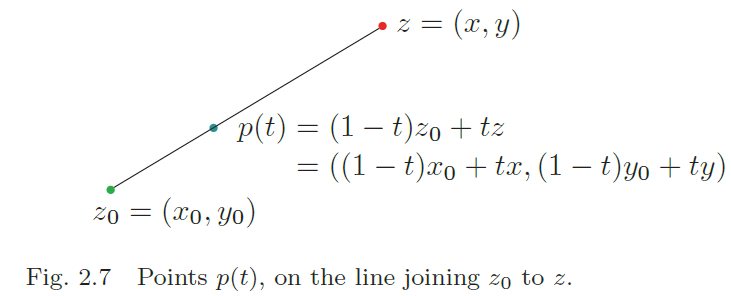
\includegraphics[width=0.6\textwidth]{./SaltChapter/fig-2-7}
\end{center}
\caption{$z_0$와 $z$를 잇는 직선 위의 점 $p(t)$}
\label{fig-2-7}
\end{figure}

함수 $\varphi_1, \varphi_2 : (-1,1) \to \mathbb R$을
\[
\begin{bmatrix}
\varphi_1(t) \\
\varphi_2(t)
\end{bmatrix}
:= 
\begin{bmatrix}
u(p(t)) \\
v(p(t))
\end{bmatrix}
\]
로 정의하자.
연쇄법칙을 적용하면
\[
\begin{bmatrix}
\varphi_1'(t) \\
\varphi_2'(t)
\end{bmatrix}
:= 
\begin{bmatrix}
\dfrac{\partial u}{\partial x}(p(t))\cdot (x-x_0) + \dfrac{\partial u}{\partial y}(p(t))\cdot (y-y_0) \\
\dfrac{\partial v}{\partial x}(p(t))\cdot (x-x_0) + \dfrac{\partial v}{\partial y}(p(t))\cdot (y-y_0) 
\end{bmatrix}.
\]
이제 새로운 표기법을 위해 아래 두 함수를 정의하자.  %## [salt] 의역 
\begin{align*}
A(t) &:= \dfrac{\partial u}{\partial x}(p(t)) = \dfrac{\partial v}{\partial y}(p(t)), \\
B(t) &:= - \dfrac{\partial u}{\partial y}t(p(t)) = \dfrac{\partial v}{\partial x}(p(t))
\end{align*}
여기서 맨오른쪽 등호는 코시-리만 방정식을 적용한 결과이다.
이제 이 표기법으로부터
\[
\begin{bmatrix}
\varphi_1'(t) \\
\varphi_2'(t)
\end{bmatrix}
:= 
\begin{bmatrix}
A(t) (x-x_0) - B(t) (y-y_0) \\
B(t) (x-x_0) + A(t) (y-y_0) 
\end{bmatrix}
= 
\begin{bmatrix}
\Re(A(t)+iB(t)) (z-z_0)) \\
\Im(A(t)+iB(t)) (z-z_0)) 
\end{bmatrix}
\]
를 얻으며,
\begin{align*}
f(z) - f(z_0) 
&= u(x,y) - u(x_0, y_0) + i (v(x,y) - v(x_0, y_0)) \\
&= \varphi_1(1) - \varphi_1(0) + i(\varphi_2(1) - \varphi_2(0)) \\
&= \int_0^1 \varphi_1'(t)dt + i\int_0^1 \varphi_2'(t)dt \\
&= \left( \int_0^1 A(t)dt + i \int_0^1 B(t)dt \right) \cdot (z-z_0).
\end{align*}
정리하면
\begin{align*}
\dfrac{f(z)-f(z_0)}{z-z_0} 
&- \left( \dfrac{\partial u}{\partial x}(x_0,y_0) 
+ i \dfrac{\partial v}{\partial x}(x_0,y_0) \right) \\
&= \int_0^1 \left( \dfrac{\partial u}{\partial x}(p(t)) 
- \dfrac{\partial u}{\partial x}(p(0)) \right)dt 
+ i \int_0^1 \left( \dfrac{\partial v}{\partial x}(p(t)) 
- \dfrac{\partial v}{\partial x}(p(0)) \right)dt.
\end{align*}
식 \eqref{eq-2-7}로부터
\[
\left| \dfrac{f(z)-f(z_0)}{z-z_0} 
- \left( \dfrac{\partial u}{\partial x}(x_0,y_0) 
+ i \dfrac{\partial v}{\partial x}(x_0,y_0) \right) \right|
< \epsilon + \epsilon = 2\epsilon
\]
이 $0<|z-z_0|<\delta$를 만족하는 모든 $z$에 대하여 성립한다.
따라서 $f$는 $z_0$에서 복소미분가능하고
\[
f'(z_0) = \dfrac{\partial u}{\partial x}(x_0,y_0) 
+ i \dfrac{\partial v}{\partial x}(x_0,y_0) 
\]
가 되어 증명이 끝난다.
\hfill $\square$

예제 \ref{exampl:example-2-1}을 다시 살펴보자.
이제는 복소미분의 정의에 사용한 $\epsilon$-$\delta$를 대신하여
위 정리로부터 제곱함수의 복소미분가능성을 확인할 수있다.

\begin{saltexample}[label=example-2-7]{}{}
함수  $f:\mathbb C \to \mathbb C$를 $f(z) = z^2$으로 정의하면
\begin{align*}
u(x,y) &= \Re(f(x+iy)) = \Re(x^2-y^2+2xyi) = x^2-y^2, \\
v(x,y) &= \Im(f(x+iy)) = \Im(x^2-y^2+2xyi) = 2xy
\end{align*}
이므로, 
\begin{align*}
\dfrac{\partial u}{\partial x}(x,y) &= 2x = \dfrac{\partial v}{\partial y}(x,y), \\
\dfrac{\partial u}{\partial y}(x,y) & -2y = - \dfrac{\partial v}{\partial x}(x,y)
\end{align*}
로부터 $\mathbb C$ 전체에서 코시-리만 방정식이 성립함을 알 수 있다.
따라서 앞에서 보인 바와 같이 $f$는 전해석함수가 된다.
또한, 
\[
f'(z) = \dfrac{\partial u}{\partial x}(x,y) + i\dfrac{\partial v}{\partial x}
= 2x + 2yi = 2z
\]
이므로 모든 $z\in\mathbb C$에 대하여 $f'(z) = 2z$이다.
\hfill $\diamondsuit$
\end{saltexample}

%\begin{saltexample}[label=example-2-8]{전해석함수}{}
\begin{saltexample}[label=example-2-8]{$\exp$, $\sin$, $\cos$\,은 전해석함수이다}{}
%\textbf{[$\exp$, $\sin$, $\cos$은 전해석함수이다]}

함수 $g:\mathbb C \to \mathbb C$를 $g(z) = \exp z$로 정의하면,
\begin{align*}
u(x,y) &= \Re(g(x+iy)) = \Re(e^x(\cos y + i\sin y)) = e^x \cos y,\\
v(x,y) &= \Im(g(x+iy)) = \Im(e^x(\cos y + i\sin y)) = e^x \sin y
\end{align*}
이므로, 
\begin{align*}
\dfrac{\partial u}{\partial x}(x,y) &= e^x\cos y 
= \dfrac{\partial v}{\partial y}(x,y), \\
\dfrac{\partial u}{\partial y}(x,y) & -e^x\sin y 
= - \dfrac{\partial v}{\partial x}(x,y)
\end{align*}
로부터 $\mathbb C$ 전체에서 코시-리만 방정식이 성립함을 알 수 있다.
따라서 $\exp$ 함수가 전해석이라는 중요한 결론에 도달한다.
또한, 
\[
g'(z) = \dfrac{\partial u}{\partial x}(x,y) + i\dfrac{\partial v}{\partial x}
= e^x\cos y + i e^x\sin y = \exp z
\]
이므로 모든 $z\in\mathbb C$에 대하여 $\dfrac{d}{dz}\exp z = \exp z$이다.
명제 \ref{prop-2-2}로부터 삼각함수
\[
\sin z  = \dfrac{\exp(iz) - \exp(-iz)}{2i}, \quad
\cos z = \dfrac{\exp(iz) + \exp(-iz)}2
\]
도 전해석함수이며 미분은 다음과 같다.
\begin{align*}
\dfrac{d}{dz} \sin z &= \dfrac{i\exp(iz) - (-i)\exp(-iz)}{2i}
= \dfrac{\exp(iz) + \exp(-iz)}2 = \cos z, \\
\dfrac{d}{dz} \cos z &= \dfrac{i\exp(iz)+(-i)\exp(-iz)}2
= - \dfrac{\exp(iz) - \exp(-iz)}{2i} = - \sin z.
\end{align*}
\hfill $\diamondsuit$
\end{saltexample}

\begin{saltexample}[label=example-2-9]{복소미분가능성}{} 
\textbf{[$\Log$의 복소미분가능성]} %{} \label{example-2-9}

주 로그함수가 열린집합 $\mathbb C \setminus(-\infty,0]$에서
복소미분가능함을 보이자.
주 로그함수는 더 큰 집합 $\mathbb C \setminus\{0\}$에 정의된 함수이지만
여기서는 연속함수가 될 수 없음을 앞에서 이미 보였다(실수축의 음수부분에서 불연속이다).
또한 더 작은 집합 $\mathbb C \setminus(-\infty,0]$에서는 주 로그함수가 연속임을 보였다.
이제 이 연속성을 이용하여 $\Log$가 $\mathbb C \setminus(-\infty,0]$에서
복소미분가능하고 그 미분은
\[
\dfrac{d}{dz} \Log (z) = \dfrac 1z 
\]
임을 증명하고자 한다.

우선 같지 않은 $z, z_0 \in \mathbb C \setminus(-\infty,0]$에 대하여
$\log (z) \ne \log(z_0)$이다 (왜?).
$\epsilon>0$에 대하여
\[
\epsilon_1 := \min \left\{ \dfrac{|z_0|}2, \dfrac{|z_0|^2}2\epsilon \right\}
\]
로 정한다.
$\exp w$가 $w_0:=\Log(z_0)$에서 미분가능하므로,
$0<|w-w_0| = |w - \Log(z_0)| < \delta_1$을 만족하는 모든 $w$에 대하여
다음 식이 성립하도록 하는 $\delta_1>0$이 존재한다.
\[
\left| \dfrac{\exp w - \exp w_0}{w-w_0} - \exp w_0 \right|
= \left| \dfrac{\exp w - z_0}{w - \Log(z_0)} - z_0 \right| <\epsilon_1.
\]
$\Log$가 $\mathbb C \setminus(-\infty,0]$에서
연속인 단사함수이므로
$0<|z-z_0|<\delta$이면 
\[
0 < |\Log z - \Log z_0 | < \delta_1
\]
을 만족하도록 하는 $\delta>0$가 존재한다.

이제 $w:=\Log z$, $0<|z-z_0|<\delta$로부터
$0<|w-w_0|<\delta_1$을 얻게 되어
\[
\left| \dfrac{z-z_0}{\Log z - \Log z_0} - z_0 \right| < \epsilon_1
\]
이 성립한다.
한편, 삼각부등식을 사용하면
$ \left| \dfrac{z-z_0}{\Log z - \Log z_0} \right| \ge |z_0| - \epsilon_1 
\ge \dfrac{|z_0|}2$이다.
따라서 
$0<|z-z_0|<\delta$를 만족하면 다음 부등식이 성립한다.
\begin{align*}
\left| \dfrac{\Log z - \Log z_0}{z-z_0} - \dfrac1{z_0} \right|
&= \left| \left(z_0 - \dfrac{z-z_0}{\Log z - \Log z_0} \right)\cdot
\dfrac1{\dfrac{z-z_0}{\Log z - \Log z_0}}\cdot \dfrac1{z_0} \right| \\
&= \left| z_0 - \dfrac{z-z_0}{\Log z - \Log z_0} \right| \cdot
\dfrac1{\left|\dfrac{z-z_0}{\Log z - \Log z_0}\right|} \cdot
\dfrac1{|z_0|} \\
&< \epsilon_1 \cdot \dfrac1{|z_0|/2}\cdot \dfrac1{|z_0|} 
= \dfrac{2\epsilon_1}{|z_0|^2} < \epsilon.
\end{align*}
이상에서 $\Log$가 $\mathbb C \setminus (-\infty,0]$에서 복소미분가능하고
$\dfrac{d}{dz}\Log z = \dfrac 1z$임을 보였다.
\hfill $\diamondsuit$
\end{saltexample}

\begin{saltexample}[label=example-2-10]{}{}
다음과 같이 정의된 함수 $f:\mathbb C \to \mathbb C$를 생각하자.
\[
x+iy\ne0 \text{ 에 대하여 } f(x+iy) = \dfrac{xy(x+iy)}{x^2+y^2} \text{ 이고,}\quad f(0)=0.
\]
$0$이 아닌 $(x,y)\in\mathbb R$에 대하여
\begin{align*}
u(x,y) &= \Re(f(x+iy)) = \dfrac{x^2y}{x^2+y^2}, \\
v(x,y) &= \Im(f(x+iy)) = \dfrac{xy^2}{x^2+y^2}
\end{align*}
이고 $u(0,0) = v(0,0) = 0$이다.
따라서,
\[
\dfrac{\partial u}{\partial x}(0,0) = 0 = \dfrac{\partial v}{\partial y}(0,0),
\quad
\dfrac{\partial u}{\partial y}(0,0) = 0 = -\dfrac{\partial v}{\partial x}(0,0)
\]
로부터 $(0,0)$에서 코시-리만 방정식이 만족된다.
하지만, 함수 $f$는 $0$에서 복소미분가능하지 않다.

만약 미분가능하다면,
\[
f'(0) = \dfrac{\partial u}{\partial x}(0,0)  + i \dfrac{\partial v}{\partial x}(0,0)  
= 0+ i0 =0
\]
이 되어야 한다. $\epsilon=1/4$로 잡으면
대응하는 $\delta$가 존재하여
$0<|z-0| = |x+iy| <\delta$이면
\[
\left| \dfrac{f(z)-f(0)}{z-0} - f'(0) \right| = \left| \dfrac{xy}{x^2+y^2} \right| < \epsilon
\]
이 항상 성립해야 한다.
하지만, $x+iy = \dfrac\delta 2 + i\dfrac\delta 2$로 택하면
\[
\dfrac12 = \left| \dfrac{xy}{x^2+y^2} \right| < \epsilon = \dfrac 14
\]
가 되어 모순이 생긴다. 따라서 $f$는 $0$에서 복소미분 불가능이다.

$u$가 $(0,0)$에서 미분가능하지 않기 때문에
정리 \ref{thm-2-2}와 모순되지는 않는다.
만약 $u$가 미분가능하다면 $(0,0)$에서의 미분은 선형변환
\[
\begin{bmatrix}
x\\ y
\end{bmatrix}
\mapsto
\begin{bmatrix}
\dfrac{\partial u}{\partial x}(0,0) & \dfrac{\partial u}{\partial y}(0,0)
\end{bmatrix}
\begin{bmatrix}
x\\ y
\end{bmatrix}
=
\begin{bmatrix}
0 & 0
\end{bmatrix}
\begin{bmatrix}
x\\ y
\end{bmatrix}
= 0
\]
이 된다.
그렇다면 $\epsilon:=1/3$이라 하면
$\delta>0$가 존재하여 
$0<\| (x,y) - (0,0)\|_2 < \delta$이면 다음이 성립해야 한다.
\[
\dfrac{|u(x,y) - u(0,0) - 0((x,y)-(0,0))|}{\|(x,y) - (0,0)\|_2}
= \dfrac{x^2y}{(x^2+y^2)^{\frac32}} < \epsilon = \dfrac 13.
\]
그런데 $(x,y) = \left(\dfrac\delta2,\dfrac\delta2\right)$로 택하면,
$\|(x,y) - (0,0)\|_2 = \dfrac\delta{\sqrt{2}} < \delta$이지만
\[
\dfrac{x^2y}{(x^2+y^2)^{\frac32}}
= \dfrac{\dfrac{\delta^2}4\cdot \dfrac\delta2}
{\left(\dfrac{\delta^2}4+\dfrac{\delta^2}4\right)^{\frac32}} 
= \dfrac1{\sqrt{8}} < \epsilon = \dfrac 13 = \dfrac 1{\sqrt{9}}
\]
가 되어 모순이다. 따라서 $u$는 $(0,0)$에서 미분가능하지 않다.
\footnote{미분 경로에 따라 미분값이 달라진다는 것을 보이는 방법으로도
같은 결과를 얻을 수 있다.}
\hfill $\diamondsuit$
\end{saltexample}

코시-리만 방정식은 몇가지 흥미로운 사실들의 증명에도 사용된다.
다음 예제는 앞에서 미리 언급했던 복소미분의 ``엄밀성''을 보여준다.
연습문제 \ref{ex-2-12}에서도 엄밀성을 엿볼 수 있다.


\begin{saltexample}[label=example-2-11]{}{}
\textbf{[절대값이 일정한 복소미분가능 함수는 상수함수이다]}  %{} \label{example-2-11}

원판 $D=\{ z\in\mathbb C \,:\, |z-z_0| <r \}$을 생각하자.
코시-리만 방정식의 응용하면 복소미분가능함수 $f: D \to \mathbb C$가
모든 $z\in D$에 대하여 $|f(z)| =c$를 만족하는 상수 $c\in\mathbb R$가 
존재한다면 $f$는 상수함수임을 보이자 
(이 결과는 나중에 ``최대 절대값 정리(Maximum Modulus Theorem)''라 불리는 결과를
학습할 때 사용할 것이다).
아래 그림을 보자.

%\begin{figure*}[!h]
\begin{center}
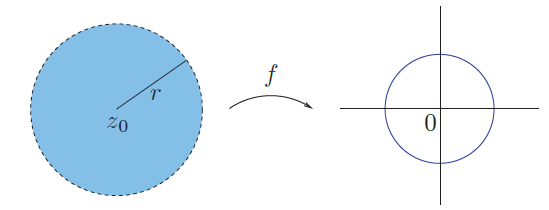
\includegraphics[width=0.6\textwidth]{./SaltChapter/fig-2-0-2}
\end{center}
%\end{figure*}

$u$, $v$를 각각 $f$의 실수부와 허수부라 하자. 
가정에서 $c^2=|f|^2 = u^2 + v^2$임을 알 수 있고 이를 미분하면,
\begin{align*}
u\dfrac{\partial u}{\partial x} + v\dfrac{\partial v}{\partial x} &= 0, \\
u\dfrac{\partial u}{\partial y} + v\dfrac{\partial v}{\partial y} &= 0.
\end{align*}
처음 방정식에 $\dfrac{\partial v}{\partial x} = - \dfrac{\partial u}{\partial y}$를
두번째 방정식에 $\dfrac{\partial v}{\partial y} = \dfrac{\partial u}{\partial x}$를
적용하면
\begin{eqnarray}
u\dfrac{\partial u}{\partial x} - v\dfrac{\partial u}{\partial y} &= 0, \label{eq-2-8}\\
u\dfrac{\partial u}{\partial y} + v\dfrac{\partial u}{\partial x} &= 0. \label{eq-2-9}
\end{eqnarray}

$\dfrac{\partial u}{\partial y}$를 소거하기 위해 식 \eqref{eq-2-8}에 $u$를 곱하고
식 \eqref{eq-2-9}에 $v$를 곱하여 더하면
$(u^2+v^2)\dfrac{\partial u}{\partial x}  = 0$을
$\dfrac{\partial u}{\partial x}$를 소거하기 위해 식 \eqref{eq-2-8}에 $-v$를 곱하고
식 \eqref{eq-2-9}에 $u$를 곱하여 더하면
$(u^2+v^2)\dfrac{\partial u}{\partial y}  = 0$을 얻는다.
$c=0$이면  $u^2+v^2=c^2=0$이 되어 $u=v=0$이므로 $D$에서 $f=0$이 된다.
$c\ne0$이면 $\dfrac{\partial u}{\partial x}= \dfrac{\partial u}{\partial y}=0$이고
코시-리만 방정식을 적용하면 
$\dfrac{\partial v}{\partial x}= \dfrac{\partial v}{\partial y}=0$도 얻는다.
적분의 기본정리로부터 
\begin{align*}
u(x,y_0) - u(x_0, y_0) &= \int_{x_0}^x \dfrac{\partial u}{\partial x}(\xi, y_0)d\xi, \\
u(x,y) - u(x, y_0) &= \int_{y_0}^y \dfrac{\partial u}{\partial y}(x, \eta)d\eta
\end{align*}
를 얻고, 임의의 점 $(x,y)$에서 $u$는 $z_0 = (x_0,y_0)$에서와 같은 값을 갖게 되어
 $u$는 $D$에서 상수이다.

%\begin{figure*}[!h]
\begin{center}
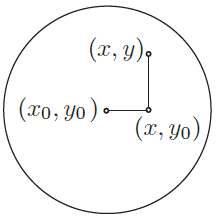
\includegraphics[width=0.25\textwidth]{./SaltChapter/fig-2-0-3}
\end{center}
%\end{figure*}

비슷한 방법으로 $v$가 $D$에서 상수임을 보일 수 있어
결론적으로 $f=u+iv$가 $D$에서 상수함수이다.
\hfill $\diamondsuit$
\end{saltexample}

\begin{salt_exercise} \label{ex-2-10}
코시-리만 방정식을 이용하여 $z\mapsto z^3$이 전해석함수임을 보여라.
\end{salt_exercise}

\begin{salt_exercise} \label{ex-2-11}
$z\mapsto \Re(z)$는 어떤 점에서도 복소미분가능하지 않음을 증명하라.
\end{salt_exercise}

\begin{salt_exercise} \label{ex-2-12}
$D$가 복소평면 $\mathbb C$의 영역이라 하자.
코시-리만 방정식을 이용하여 
$D$에 정의된 복소해석함수 $f:D\to\mathbb C$가 
모든  $z\in D$에 대하여 $f(z)\in\mathbb R$이면
$f$는 $D$에서 상수함수임을 보여라.
\end{salt_exercise}

\begin{salt_exercise} \label{ex-2-13}
$D$가 복소평면 $\mathbb C$의 영역이라 하자.
$D$에 정의된 복소해석함수 $f:D\to\mathbb C$가 
모든  $z\in D$에 대하여 $f'(z)=0$이면
$f$는 $D$에서 상수함수임을 보여라.
\end{salt_exercise}

\begin{salt_exercise} \label{ex-2-14}
전해석함수 $f:\mathbb C \to \mathbb C$에 대하여
$u:=\Re(f)$, $v:=\Im(f)$라 하자.
$u= h\circ v$를 만족하는 미분가능함수 $h:\mathbb R \to \mathbb R$가
존재한다면 $f$는 상수함수임을 보여라.
\end{salt_exercise}

\begin{salt_exercise} \label{ex-2-15}
고정된 상수 $k\in\mathbb R$가 주어졌을 때
모든 $z=x+iy$ ($x,y\in \mathbb R$)에 대하여 $f(z)=(x^2-y^2) +kxyi$로 정의하자.
$f$가 전해석함수일 필요충분조건은 $k=2$임을 보여라.
\end{salt_exercise}

\section{복소미분의 기하학적 의미\label{sec-2-3}}

미분의 기본을 공부할 때, 점 $x_0\in\mathbb R$에서 실변수 함수 $f:\mathbb R\to \mathbb R$의 
미분 $f'(x_0)$에 대한 기하학적 의미는 $x_0$점에서 $f$에 접하는 접선의 기울기를 의미함을
이미 배웠을 것이다. 그림 \ref{fig-2-8}을 참고하라.

\begin{figure}[!h]
\begin{center}
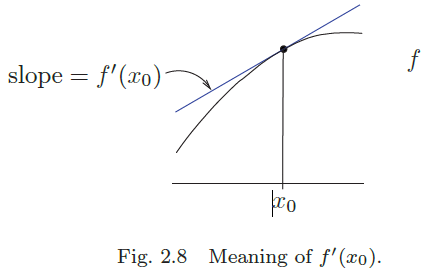
\includegraphics[width=0.5\textwidth]{./SaltChapter/fig-2-8}
\end{center}
\caption{$f'(x_0)$의 의미}
\label{fig-2-8}
\end{figure}

$\lim\limits_{x\to x_0} \dfrac{f(x) - f(x_0)}{x-x_0} = f'(x_0)$는
$x_0$ 근방의 $x$에 대하여
$\dfrac{f(x) - f(x_0)}{x-x_0} \approx f'(x_0)$임을 의미한다. 즉,
\[
f(x) - f(x_0) \approx f'(x_0)(x-x_0).
\]
국소적으로 $x_0$ 근방에서 $f(x)-f(x_0)$는 $x-x_0$에 {\bf 선형}함수 
$h \mapsto f'(x_0)h : \mathbb R \to \mathbb R$을 적용한 것으로 볼 수 있음을 의미한다.
그림으로 보면 $x_0$ 근방에서 
$(x_0, f(x_0))$를 지나고 기울기가 $f'(x_0)$인 접선과 함수 $f$의 그래프의 차이가 거의 없음을 
의미한다. 
다시 말하면, $(x_0, f(x_0))$의 근방을 확대하면   함수의 그래프는 직선과 거의 일치한다.

이 절에서는 $U$에 정의된 복소함수 $f:U \to \mathbb C$가
$z_0$에서 복소미분 가능할 때 비슷한 질문을 유추해보자.
\begin{center}
\fbox{
복소수 $f'(z_0)$의 기하학적 의미는 무엇인가?
}
\end{center}

우리가 $f$의 그래프를 그려볼 수는 없다.
왜냐 하면, $z$와 $f(z)$가 $\mathbb C = \mathbb R^2$에 속하므로
$(z, f(z))$는 $\mathbb R^2 \times \mathbb R^2 = \mathbb R^4$의 점이 되기 때문이다.
하지만 아래 그림과 같이
정의역 $U$를 왼쪽 평면에 공역 $\mathbb C$를 오른쪽에 놓고
$f$가 왼쪽 $U$의 한점을 오른쪽으로 보내는 것으로 그려볼 수 있다.

\begin{figure*}[!h]
\begin{center}
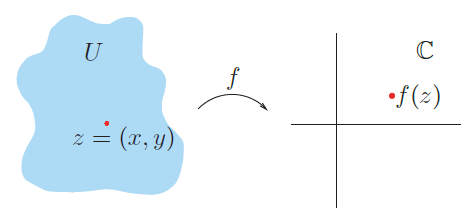
\includegraphics[width=0.5\textwidth]{./SaltChapter/fig-2-0-4}
\end{center}
\end{figure*}

복소수 $f'(z_0)$를 
$z_0$의 근방에서 국소적으로 보면 
복소미분가능함수를 반시계방향으로 각도 $\Arg(f'(z_0))$만큼 회전시키고
$|f'(z_0)|$만큰 확대시키는 것임을 보이도록 하자.

$\lim\limits_{z\to z_0} \dfrac{f(z) - f(z_0)}{z-z_0} = f'(z_0)$는
$z_0$ 근방의 $z$에 대하여
$\dfrac{f(z) - f(z_0)}{z-z_0} \approx f'(z_0)$임을 의미한다. 즉,
\[
f(z) - f(z_0) \approx f'(z_0)(z-z_0).
\]

복소수 곱셈의 기하학적 의미로부터
$z-z_0$에 $f'(z_0)$를 곱하는 것은
$z-z_0$를 각도 $\Arg(f'(z_0))$만큼 반시계방향으로 회전시키고,
$z-z_0$의 길이는  $f'(z_0)$의 길이를 곱하는 것임을 알고 있다. 즉, $|f'(z_0)|$만큼 확대한 것이다.
이를 잘 이해하기 위해 그림 \ref{fig-2-9}를 참고하자.

\begin{figure}[!h]
\begin{center}
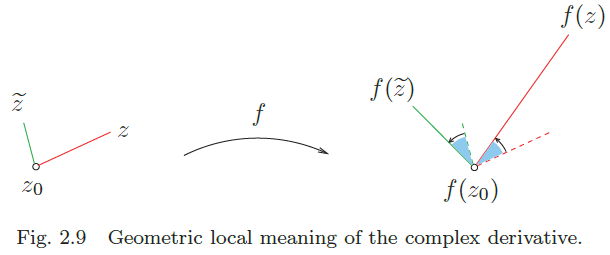
\includegraphics[width=0.8\textwidth]{./SaltChapter/fig-2-9}
\end{center}
\caption{국소적으로 본 복소미분의 기하학적 의미}
\label{fig-2-9}
\end{figure}

$f'(z_0) = \sqrt{3} +i$라고 가정하자.
그러면 $|f'(z_0)| = 2$이고 $\Arg(f'(z_0))=\pi/6$이다.
영역 $D$의 내부에서 $z-z_0$는 $z$와 $z_0$를 잇는 선분으로 볼 수 있다.
오른쪽 그림에 이를 평행이동시킨 선분을 $f(z_0)$에서 출발하는 점선으로 표시하였다.
$f(z)$의 위치를 찾기 위해서는
$f(z)-f(z_0)$는 $f'(z_0)$에 $z-z_0$를 곱한 것과 근사적으로 같다는 것을 이용한다.
오른쪽 그림에서 실선으로 표시된 $f(z)-f(z_0)$는
점선을 각도 $\Arg(f'(z_0))$만큼 반시계방향으로 회전시켜 얻는다
(이 그림에서는 $30^\circ$로 가정하였다).
또한 길이는 점선의 길이를 $|f'(z_0)|=2$만큼 확대하여 얻는다.
$z_0$ 근방의 다른 점 $\tilde z$에 대한 이미지를 얻기 위해서는 
같은 과정을 반복하면 된다.
즉, 먼저 $z_0$와  $\tilde z$를 잇는 선분을 왼쪽에 실선으로 그린다.
평행이동시킨 선분을 $f(z_0)$에서 출발하는 점선으로 오른쪽에 표시한다.
$f(\tilde z)$의 위치를 찾기 위해
점선을 $f'(z_0)$의 편각, 즉, $30^\circ$만큼 반시계방향으로 회전시키고
점선의 길이를 $|f'(z_0)|=2$만큼 확대한 실선을 그린다.
이를 통해 $f(\tilde z) - f(z_0)$를 표현하는 실선을 얻고
한쪽 끝을 $f(z_0)$ 에 두면 다른 쪽은 $f(\tilde z)$를 얻는다 (근사적으로!).
따라서 $f$의 국소적인 영향을 다름과 같이 정리할 수 있다.
영역을 고무판으로 간주하고 고무판 위에 점 $z_0$를 관찰하자.
$z_0$ 주변의 작은 부분을 뜯어내자.
함수 $f$는 고무판 위의 점 $z_0$를 복소평면 위 어딘가에 있는 $f(z_0)$로 보낸다.
뜯어진 작은 고무판위의 다른 점들은 $f$에 의해 어떤 점으로 가는지를
알아보려면 다음 과정을 따른다.
복소평면의 $f(z_0)$의 바로 위에 $z_0$가 올려지도록 고무판을 위치시킨다
(뜯어진 작은 고무판 위의 점 $z_0$에 핀을 꽂아 평면 위에 고정시킨다고 상상하자).
이제 $z_0$를 중심으로 하여 $|f'(z_0)|$의 배율로 고무판을 당기고,
당겨진 고무판을 $z_0$ 주변으로 각도 $\Arg(f'(z_0))$만큼 반시계방향으로 회전시킨다.

기하학적 해석을 강조하기 위해
제곱함수 $z\mapsto z^2$을 다루는
예제 \ref{example-2-1}를 다시 생각해보자.
그림 \ref{fig-2-10}과 예제 \ref{example-2-12}를 참고하자.

\begin{figure}[!h]
\begin{center}
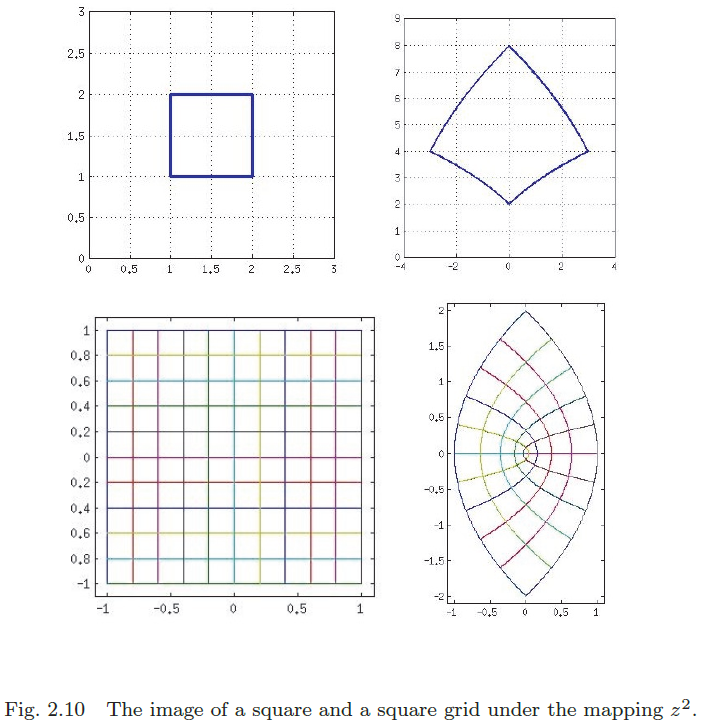
\includegraphics[width=0.8\textwidth]{./SaltChapter/fig-2-10}
\end{center}
\caption{함수 $z^2$에 의한 정사각형과 사각 격자의 상}
\label{fig-2-10}
\end{figure}

\begin{saltexample}[label=example-2-12]{}{}
점 $z_0\in\mathbb C$에서 제곱함수  $z\mapsto z^2$의
복소미분가능성을 가정하자.
$z_0$ 근방에서 제곱함수에 의한  국소 확대와 국소 회전을 기하학적으로 이해함으로써
$z_0$에서 제곱함수의 복소미분이 $2z_0$가 되어야 함을 증명하도록 하자.

첫번째 질문:국소 회전은 얼마나 되는가?
이를 찾기 위해 $z_0$에 가까운 점 $z$와 $z_0$에서 $z$를 잇는 반직선이 원점을 지난다고하자.
\footnote{반직선이 `원점'을 지난다는 조건이 필요하다}
그림 \ref{fig-2-11}은 제곱함수의 영향을 나타낸다. 즉, 편각은 두배가 되고
원점에서의 거리는 제곱이 된다. 
 $z^2$은 원점과 
실수축의 양의 방향과 이루는 각이 $2\Arg(z_0)$인
$z_0^2$을 잇는 반직선 위에 있다.
따라서 $z_0^2$과 $z^2$을 잇는 선분은 
$z_0$와  $z$를 잇는 선분을 $\Arg(z_0)$만큼 반시계방향으로 회전시켜 얻을 수 있다. 
\footnote{회전시킨 후 선분의 길이도 조정해야 한다}
결론적으로  $\Arg(f'(z_0)) = \Arg(z_0)$이다.

%\begin{figure}[!h]
\begin{center}
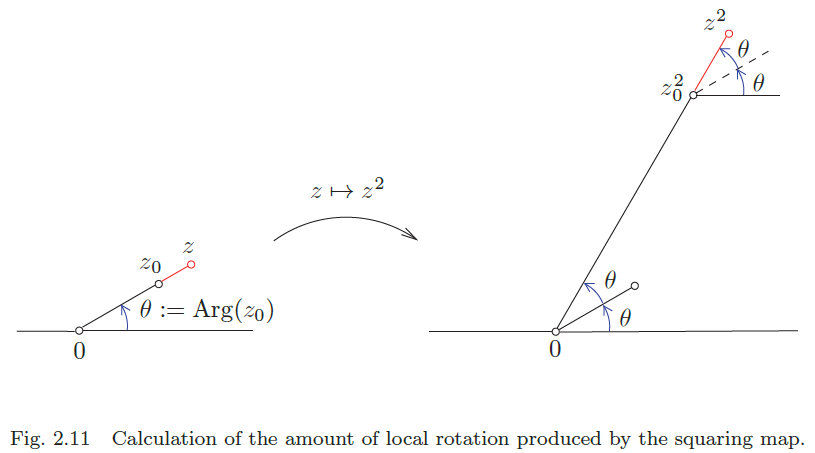
\includegraphics[width=0.7\textwidth]{./SaltChapter/fig-2-11}
\end{center}
\captionof{figure}{제곱함수에 의한 국소 회전량의 계산}
\label{fig-2-11}
%\end{figure}


다음 질문: 확대 비율은 얼마인가?
이를 찾기 위해 $z_0$에 가까운 점 $z$가 다음 조건을 만족하도록 선택한다.
$z$는 원점에서의 거리가 $z_0$와 같으며 
실수축의 양의 방향과 이루는 각은 $\theta + d\theta$로 약간 크다.
그림 \ref{fig-2-12}에 표현된 제곱함수의 성질을 보면,
$d\theta$가 작은 값이기 때문에 근사적으로 길이 $|z-z_0|$는  $|z_0|\cdot d\theta$이고,
길이 $|z^2-z_0^2|$은 $|z_0|^2\cdot 2d\theta$이다.
결론적으로 확대비율 $|f'(z_0)|$는 $(|z_0|^2\cdot 2d\theta)/(|z_0|\cdot d\theta) = 2|z_0|$이다.


%\begin{figure}[!h]
\begin{center}
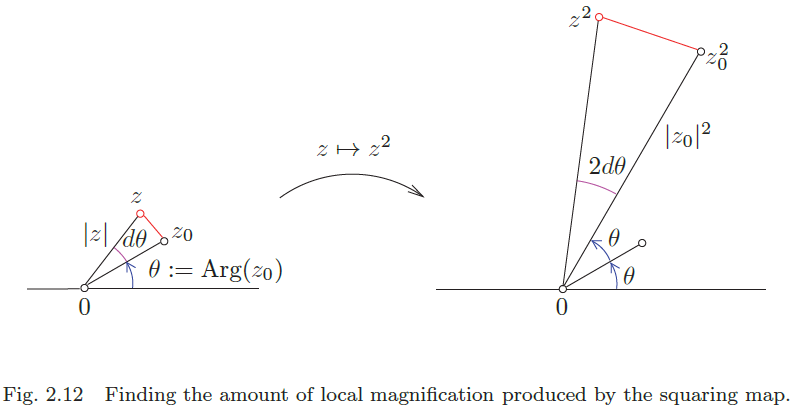
\includegraphics[width=0.7\textwidth]{./SaltChapter/fig-2-12}
\end{center}
\captionof{figure}{제곱함수에 의한 국소 확대 배율의 계산}
\label{fig-2-12}
%\end{figure}

종합하면,
\begin{align*}
f'(z_0) &= |f'(z_0)| \cdot
\left( \cos(\Arg(f'(z_0))) + i \sin(\Arg(f'(z_0))) \right) \\
&= 2|z_0|\cdot \left(\cos(\Arg(z_0)) + i \sin(\Arg(z_0)) \right) \\
&= 2z_0
\end{align*}
이고,
$z_0$ 근방에서 제곱함수 $f$의 국소적 성질을 조사함으로써
복소미분 $f'(z_0)$를 구할 수 있다.
\hfill $\diamondsuit$
\end{saltexample}

\begin{saltexample}[label=example-2-13]{켤레복소수 함수는 어떤 점에서도 복소미분이 불가능하다}{}
그림 \ref{fig-2-13}을 보자.

%\begin{figure}[!h]
\begin{center}
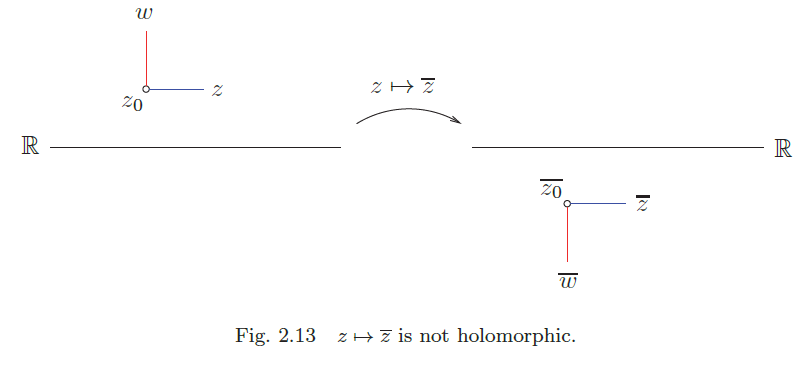
\includegraphics[width=0.8\textwidth]{./SaltChapter/fig-2-13}
\end{center}
\captionof{figure}{$z\mapsto \bar z$는 복소미분가능하지 않다}
\label{fig-2-13}
%\end{figure}

$z\mapsto \bar z$가 $z_0$에서 복소미분가능하다고 가정하자.
그러면 $z_0$ 근방에서 함수는 국소적으로 회전과 확대를 나타낸다.
$z$를 $z_0$에서 수평으로 약간 평행이동한 점이라고 하자.
그림에서 $\overline{z_0}$와 $\bar z$를 보면
$\bar z - \overline{z_0} = z-z_0$이므로 회전은 일어나지 않는다.
한편 $w$를 $z_0$를 수직방향으로 약간 이동한 점이라고 하면
그림에서 $\bar w - \overline{z_0} =  - (w-z_0)$이므로
$180^\circ$의 회전이 일어났다.
그런데 국소적으로 함수는 회전을 나타내지 못한다
(회전을 나타낸다면 $z_0$를 중심으로 하는  작은 벡터 {\bf 모두}에 대하여 
$f$가 동일한 양의 회전을 보여여한다).
\hfill $\diamondsuit$
\end{saltexample}

\begin{salt_exercise}\label{ex-2-16}
우리는 거듭제곱 함수 $z\mapsto z^n$ ($n\in\mathbb N$)가 전해석함수임을 알고 있다.
국소적 성질을 조사하는 방법으로 이 함수의 복소미분을 구하라. \\[1ex]
힌트:  $z_0$를 중심으로 하는  작은 벡터 모두에 대하여
회전과 확대가 동일하기 때문에
원점과 $z_0$를 있는 반직선에 수직인 작은 벡터에 대하여 
예제 \ref{example-2-12}를 적용하면 간단히 결론을 얻을 수 있다.
\end{salt_exercise}

\begin{salt_exercise}\label{ex-2-17}
우리는 거듭제곱 함수 $z\mapsto e^z$가 전해석함수임을 알고 있다.
국소적 성질을 조사하는 방법으로 이 함수의 복소미분을 구하라. \\[1ex]
힌트:  점 $z_0$를 위쪽으로 거리 $\delta$만큼 이동시키고
함수를 적용한 결과로부터 확대 배율을 결정하라.
비슷한 방법으로 
점 $z_0$를 수평으로 $\delta$만큼 이동시키고
국소적인 회전량을 결정하라.
\end{salt_exercise}

\begin{salt_exercise}\label{ex-2-18}
함수 $z\mapsto \Re(z)$가 
$\mathbb C$의 어떤 점에서도 복소미분가능하지 않음을 보이기 위하여
그림을 이용하는 방법을 제시하라.
\end{salt_exercise}

{\bf 등각성(comformality):}
전해석함수 $\exp$를 표현한 그림 \ref{fig-1-16}을 다시 보자.
이 그림에서 정의역에 있는 수직선과 수평선은 함수로 보낸 이미지도
다시 서로 수직이 됨을 알 수 있다.
이미 언급했었지만 이러한 특성을 등각성이라 한다.
즉, 모든 복소미분가능 함수는 정의역에서 두 곡선이 이루는 각도를 ``방향''과 함께 
보존한다. 이는 모든 복소해석함수가 갖는 성질임을 이미 언급했었다.
이제 복소해석함수가 왜 이런 성질을 갖는지 그 이유를
앞에서 학습한 복소미분가능함수의 국소적 성질을 바탕으로 규명해보자.

\begin{figure}[!h]
\begin{center}
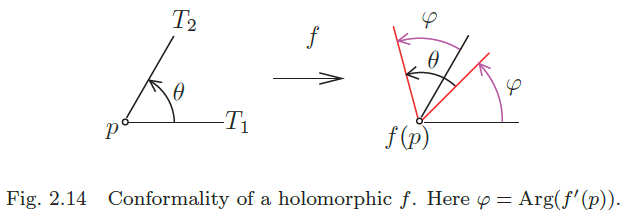
\includegraphics[width=0.8\textwidth]{./SaltChapter/fig-2-14}
\end{center}
\caption{복소해석함수 $f$의 등각성.  $\varphi = \Arg(f'(p))$}
\label{fig-2-14}
\end{figure}

$f: U\to \mathbb C$가 복소해석함수라 하고,
점 $p\in U$에서 교차하는 두 개의 매끄러운 곡선을 생각하자.
곡선들은 미분가능하므로 $p$에서 접선 $T_1$, $_2$를 갖는다.
그림 \ref{fig-2-14}를 보자. 
$p$ 근방에서는 곡선과 접선의 차이가 거의 없기 때문에
곡선을 접선으로 간주할 수 있다.
이제 이 접선들이 이루는 각을 생각할 수 있는데  $f$가 접선에 대하여 어떤 작용을 하는지 살펴보자.
곡선들은 $f$에 의해 $f(p)$에서 교차하는 새로운 곡선으로 변환된다.
변환된 결과도 매끄러운 곡선이며 접선을 갖는다.
한편 $p$ 근방에서 $f$의 국소적 변환은 $\Arg(f'(p))$ 만큼 반시계방향으로 회전시키고
확대하는 것이므로, 변환된 곡선의 접선은
정의역의 접선을 회전시키고 확대한 결과이다.
당연히 두 접선을 동일한 각도로 회전시키며 방향도 동일하게 유지한다.
따라서 복소해석함수의 등각성은 이제 더 이상 신기한 특징이 아니다!

{\bf 실함수 미분가능성과의 관계, 코시-리만 방정식의 재고찰:}
열린집합 $U$의 한점 $z_0=(x_0,y_0)$에서
복소미분가능한 함수 $f: U\to \mathbb C$를 생각하자.
$u$, $v$를 $f$의 실수부와 허수부라 하면
$u,v:U\to \mathbb R$은 $(x_0, y_0)$에서 미분가능함을 알고 있다.
따라서 $f$를 함수 $ (x,y) \mapsto (u(x,y), v(x,y)): U\to\mathbb R^2$로 보면
미분가능하며(실변수 함수로서), 미분은 국소적으로 선형변환을 나타낸다.
\[
A:= \begin{bmatrix}
\dfrac{\partial u}{\partial x}(x_0,y_0) & \dfrac{\partial u}{\partial y}(x_0,y_0) \\
\dfrac{\partial v}{\partial x}(x_0,y_0) & \dfrac{\partial v}{\partial y}(x_0,y_0) 
\end{bmatrix}
\]
한편 $f$가 복소미분가능하므로 국소변환은 각도 $\theta:=\Arg(f'(z_0))$만큼 
반시계방향으로 회전시키고 $r:=|f'(z_0)|$의 배율로 확대한 것이다.
따라서 선형변환은 다음 행렬로 나타낼 수 있다.
\[
r\begin{bmatrix}
\cos\theta & - \sin\theta \\
\sin\theta & \cos\theta
\end{bmatrix}
\]
이 행렬이 $A$와 같아야 하므로 다음 관계식을 얻는다.
\begin{align*}
\dfrac{\partial u}{\partial x}(x_0,y_0) &= r\cos\theta = \dfrac{\partial v}{\partial y}(x_0,y_0), \\
\dfrac{\partial v}{\partial x}(x_0,y_0) &= r\sin\theta = - \dfrac{\partial u}{\partial y}(x_0,y_0).
\end{align*}
또한, 미분은
$f'(z_0) = r(\cos\theta + i \sin\theta) = 
\dfrac{\partial u}{\partial x}(x_0,y_0) +i \dfrac{\partial v}{\partial x}(x_0,y_0)$이다.

요약하면, $f$가 $z_0$에서 복소미분가능하면
실함수로서 미분도 가능하다($U\subset \mathbb R^2$에서 $\mathbb R^2$로의 함수로서).
하지만 실함수의 미분과 복소미분의 차이를 보면
실함수 미분은 단지 선형변환을 나타내지만 복소미분은 특별한 형식의 선형변환을 나타낸다.
즉, 각도 $\theta$만큼 반시계방향으로 회전하는 것과 $r$만큼의 배율로 확대하는 것을 나타낸다.

\section{d-bar 연산자}

두 개의 식으로 된 코시-리만 방정식은 다음 ``d-bar 연산자'' 개념을 도입하면
단일 방정식으로 쓸 수 있다.
\[
\dfrac\partial {\partial \bar z}
\]

미분 작용소를 다음과 같이 정의하자.
\[
\dfrac\partial {\partial z} := 
\dfrac 12 \left( \dfrac\partial {\partial x} - i \dfrac\partial {\partial y} \right),
\quad
\dfrac\partial {\partial \bar z} :=
\dfrac 12 \left( \dfrac\partial {\partial x} + i \dfrac\partial {\partial y} \right).
\]
미분 작용소는 함수에 작용하여 새로운 함수를 만든다.
예를 들어, 위의 두 미분 작용소를 
$\mathbb R^2$의 부분집합 $U$에 정의된 매끄러운 함수 $\varphi: U\to \mathbb R$에
작용시키 보자.
그러면 $\varphi$가 미분가능하기 때문에
$U$의 모든 점에서 $x$, $y$에 대한 1차 편도함수가 존재하므로 다음을 얻는다.
\[
\dfrac{\partial \varphi}{\partial z} := 
\dfrac 12 \left( \dfrac{\partial \varphi}{\partial x} 
- i \dfrac{\partial \varphi}{\partial y} \right),
\quad
\dfrac{\partial \varphi}{\partial \bar z} :=
\dfrac 12 \left( \dfrac{\partial \varphi}{\partial x} 
+ i \dfrac{\partial \varphi}{\partial y} \right).
\]
또한 $U$에 정의된 매끄러운 실변수 함수 $u$, $v$에 대하여
\[
\dfrac\partial {\partial z}(u+iv)
:= \dfrac{\partial u}{\partial z} + i\dfrac{\partial v}{\partial z},
\quad
\dfrac\partial {\partial \bar z}(u+iv)
:= \dfrac{\partial u}{\partial \bar z} + i\dfrac{\partial v}{\partial \bar z},
\]
라 정의한다.

이 표현을 따르면, 
열린집합 $U\subset \mathbb C$에 정의된 복소해석함수 $f=u+iv$에 대하여
\begin{align*}
\dfrac{\partial}{\partial \bar z} f
&= \dfrac{\partial}{\partial \bar z} (u+iv) 
= \dfrac{\partial u}{\partial \bar z} + i\dfrac{\partial v}{\partial \bar z} \\
&= \dfrac 12 \left( \dfrac{\partial u}{\partial x} 
+ i \dfrac{\partial u}{\partial y} \right)
+ i\dfrac 12 \left( \dfrac{\partial v}{\partial x} 
+ i \dfrac{\partial v}{\partial y} \right) \\
&= \dfrac 12 \left( \dfrac{\partial u}{\partial x} 
- \dfrac{\partial v}{\partial y} \right)
+ i\dfrac 12 \left( \dfrac{\partial u}{\partial y} 
+ \dfrac{\partial v}{\partial x} \right) \\
&= 0 + i0 = 0,
\end{align*}
여기서 $f$의 실수부와 허수부 $u$, $v$에 대한 코시-리만 방정식을 이용하여
마지막 등식을 얻었다.
또한, 
\begin{align*}
\dfrac{\partial}{\partial z} f
&= \dfrac{\partial}{\partial z} (u+iv) 
= \dfrac{\partial u}{\partial  z} + i\dfrac{\partial v}{\partial z} \\
&= \dfrac 12 \left( \dfrac{\partial u}{\partial x} 
- i \dfrac{\partial u}{\partial y} \right)
+ i\dfrac 12 \left( \dfrac{\partial v}{\partial x} 
- i \dfrac{\partial v}{\partial y} \right) \\
&= \dfrac 12 \left( \dfrac{\partial u}{\partial x} 
+ \dfrac{\partial v}{\partial y} \right)
+ i\dfrac 12 \left( - \dfrac{\partial u}{\partial y} 
+ \dfrac{\partial v}{\partial x} \right) \\
&= \dfrac12 \cdot 2 \dfrac{\partial u}{\partial x} 
+ i\dfrac12 \cdot 2 \dfrac{\partial v}{\partial x} 
= \dfrac{\partial u}{\partial x}  + i \dfrac{\partial v}{\partial x}  \\
&= f'.
\end{align*}
요약하면, $U$에 정의된 복소해석함수 $f$에 대하여
$\dfrac{\partial}{\partial \bar z} f =0$이고,
$\dfrac{\partial}{\partial z} f =f'$이다.

개념적으로, $z$와 $\bar z$의 함수로 볼 때
복소해석함수는  $\bar z$에 무관한 함수라고 할 수 있다.

\begin{saltexample}[label=example-2-14]{}{}
$\bar z$는 복소해석함수가 아니다. 왜냐하면,
\begin{align*}
\dfrac{\partial}{\partial \bar z}\bar z 
&= \dfrac{\partial}{\partial \bar z} (x-iy)
= \dfrac 12 \left( \dfrac\partial {\partial x} + i \dfrac\partial {\partial y} \right) x
- i \dfrac 12 \left( \dfrac\partial {\partial x} + i \dfrac\partial {\partial y} \right) y \\
&= \dfrac 12 - i\cdot \dfrac12 \cdot i = 1 \ne 0.
\end{align*}
\end{saltexample}

\begin{saltexample}[label=example-2-15]{}{}
$|z|^2 = z\bar z$는 $\mathbb C\setminus \{0\}$에서 복소해석함수가 아니다. 왜냐하면,
\begin{align*}
\dfrac{\partial}{\partial \bar z}(z \bar z)
&= \dfrac{\partial}{\partial \bar z} (x^2+y^2)
= \dfrac12 \left( \dfrac\partial {\partial x} + i \dfrac\partial {\partial y} \right) (x^2+y^2) \\
&= \dfrac 12 (2x+i2y) = x+iy = z \ne 0 \ (z\in\mathbb C\setminus \{0\}).
\end{align*}
\end{saltexample}


\begin{saltexample}[label=example-2-16]{}{}
$z^2$은 전해석함수이다. 왜냐하면,
\begin{align*}
\dfrac{\partial}{\partial \bar z}(z^2)
&= \dfrac{\partial}{\partial \bar z} (x^2-y^2 + 2xyi) \\
&= \dfrac12 \left( \dfrac\partial {\partial x} + i \dfrac\partial {\partial y} \right) (x^2-y^2) 
+ i \dfrac12 \left( \dfrac\partial {\partial x} + i \dfrac\partial {\partial y} \right) (2xy)  \\
&= \dfrac 12 (2x-i2y) + i\dfrac12(2y+i2x) = 0.
\end{align*}
또한,
\begin{align*}
\dfrac{\partial}{\partial z}(z^2)
&= \dfrac{\partial}{\partial z} (x^2-y^2 + 2xyi) \\
&= \dfrac12 \left( \dfrac\partial {\partial x} - i \dfrac\partial {\partial y} \right) (x^2-y^2) 
+ i \dfrac12 \left( \dfrac\partial {\partial x} - i \dfrac\partial {\partial y} \right) (2xy)  \\
&= \dfrac 12 (2x+i2y) + i\dfrac12(2y-i2x) = 2(x+iy)=2z.
\end{align*}
\end{saltexample}

\begin{salt_exercise} \label{ex-2-19}
$4\dfrac{\partial}{\partial z}\dfrac{\partial}{\partial \bar z} = \Delta$임을 보여라.
여기서 $\Delta := \dfrac{\partial^2}{\partial x^2} + \dfrac{\partial^2}{\partial y^2}$는
라플라스 작용소라 부른다.
\end{salt_exercise}

\section{참고}

복소미분의 기하학적 의미에 대한 부분은  [Needhan (1997)]의 설명을 따른다.
연습문제 \ref{ex-2-16}과  연습문제 \ref{ex-2-17}은 [Needhan (1997)]을 인용하였다.




